 
\subsection{One-Dimensional Discriminants}

This section contains overlayed plots of the one-dimensional (1D) $s$-channel
and $t$-channel discriminants evaluated on signal and background events. The events in
the plots come from the combination of the eight analysis channels \{$e$,$\mu$ $\oplus$ 1,2 tags $\oplus$ 2,3 jets \}. Figures~\ref{disc_wbb} and \ref{disc_wjets} show good
discrimination between signal and $W$+jets and multijets backgrounds.
However, the discrimination is poorer between signal and $\dilepton$
and $\lepjets$ events as shown in Fig.~\ref{disc_ttbar}. The lack of
discrimination power for $\ttbar$ events is due to the fact that the analysis does not yet include a $\ttbar$
probability density function in the definition of the discriminant\footnote{The $\ttbar$ matrix element takes much longer to integrate because
there are six partons in the final state while there are four in the
single top and $W$+jets matrix elements. Adding a $\ttbar$ matrix
element is envisioned as a future improvement for this analysis.}.

\begin{figure}[!h!tbp]
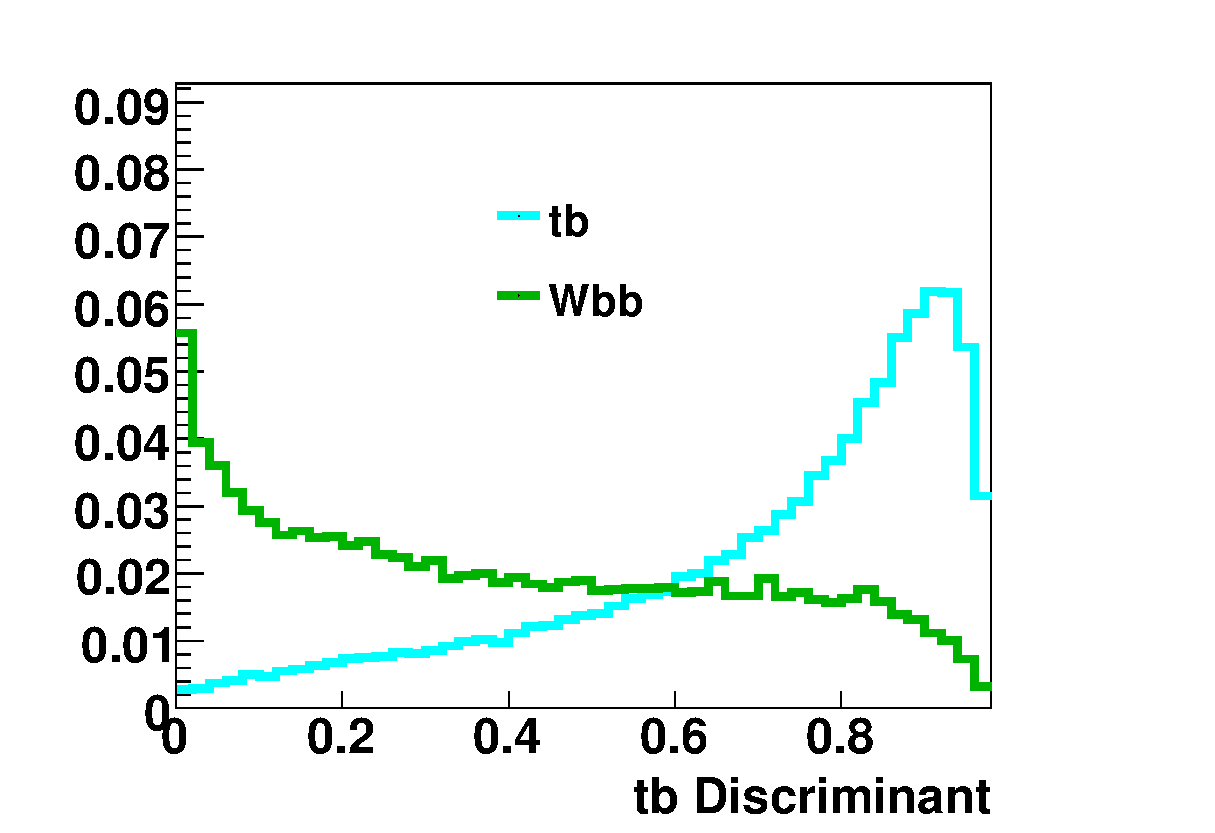
\includegraphics[width=0.49\textwidth]
{eps/MatrixElement/performance/tb_Discriminant__schannel_wbb}
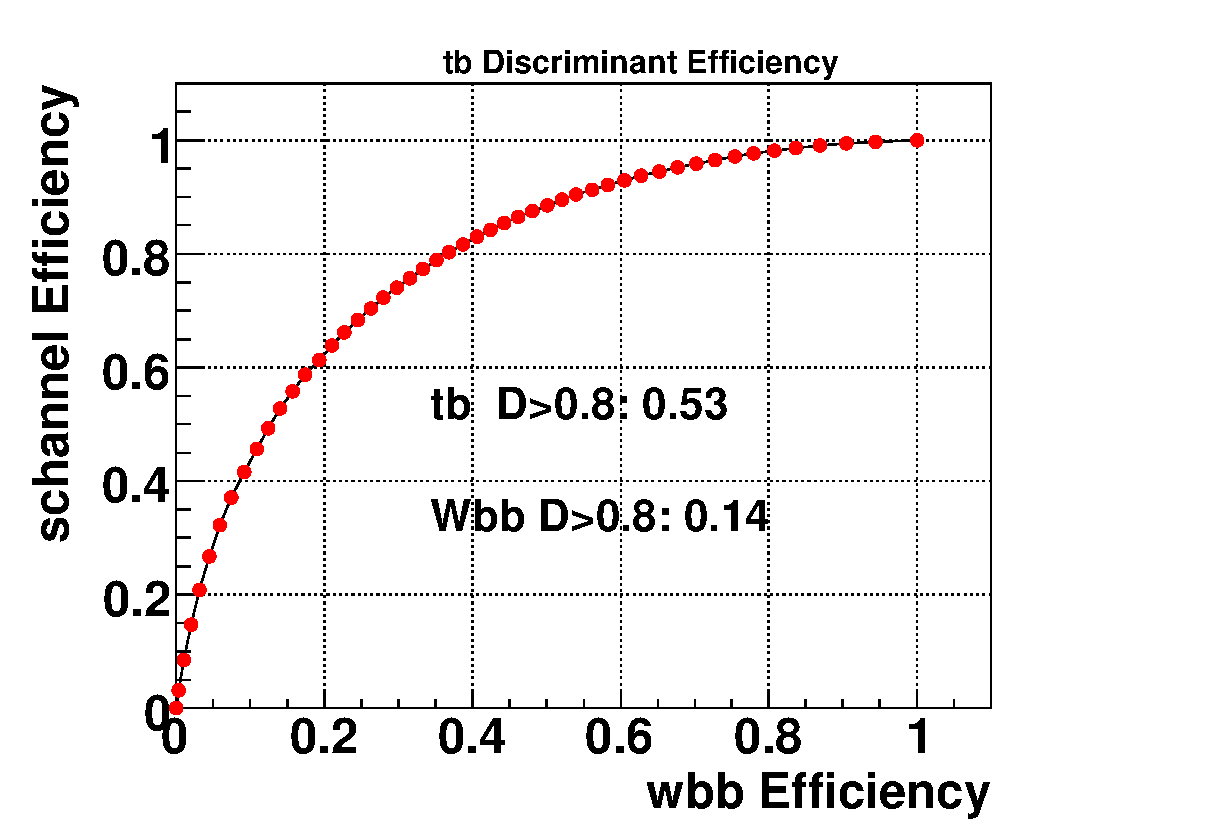
\includegraphics[width=0.49\textwidth]
{eps/MatrixElement/performance/tb_Efficiency__schannel_wbb}
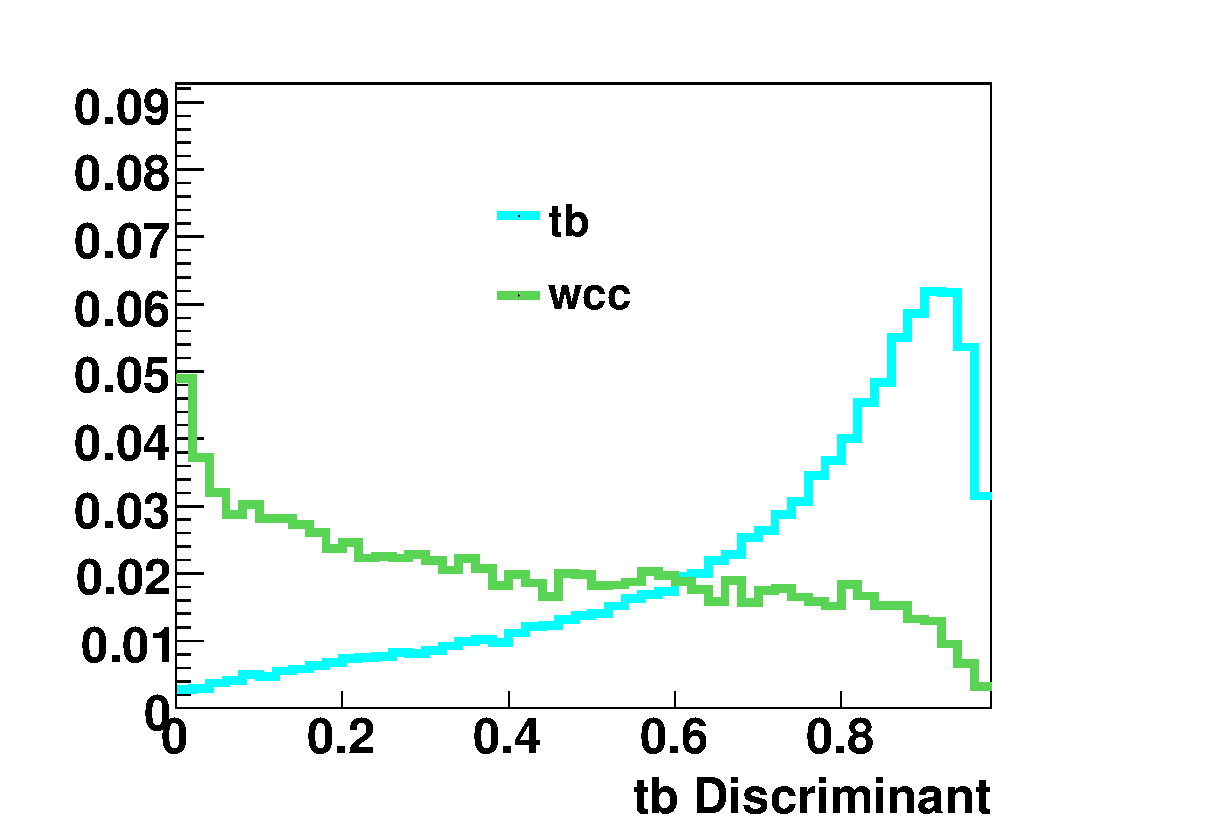
\includegraphics[width=0.49\textwidth]
{eps/MatrixElement/performance/tb_Discriminant__schannel_wcc}
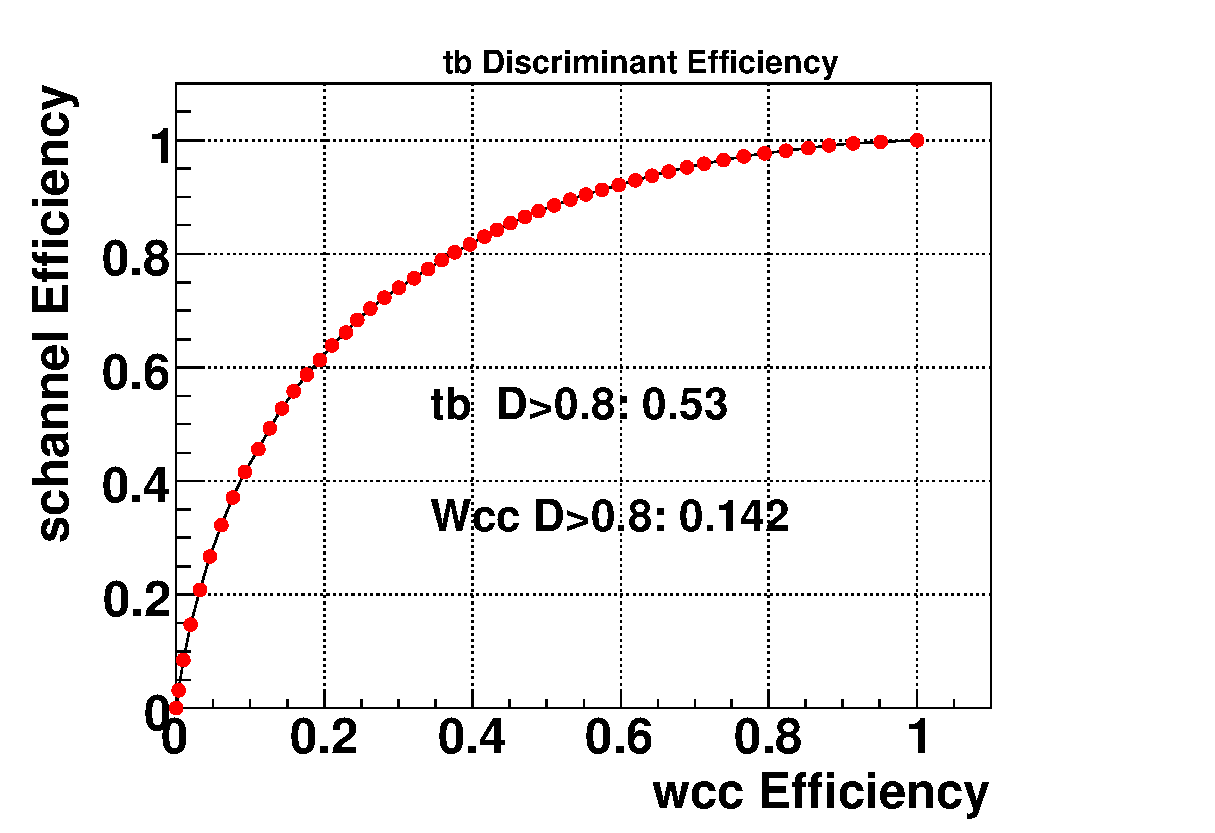
\includegraphics[width=0.49\textwidth]
{eps/MatrixElement/performance/tb_Efficiency__schannel_wcc}
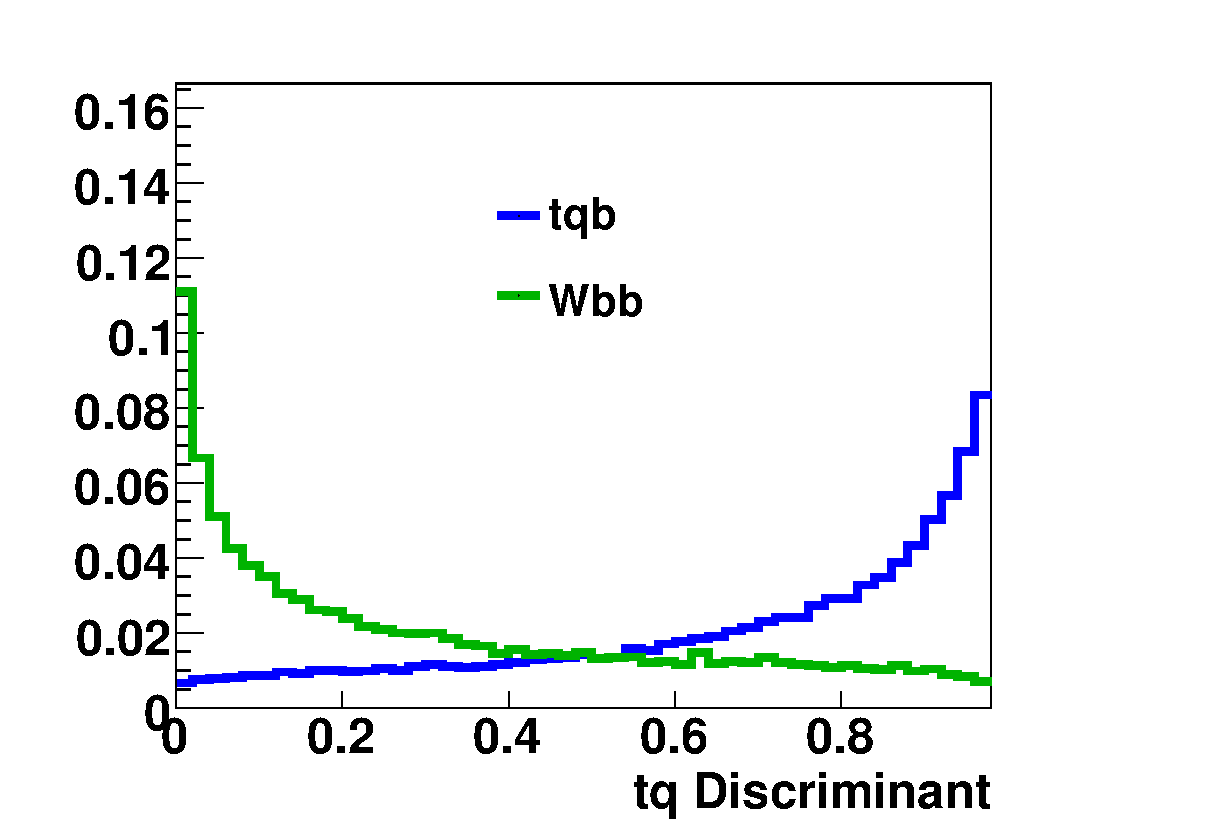
\includegraphics[width=0.49\textwidth]
{eps/MatrixElement/performance/tq_Discriminant__tchannel_wbb}
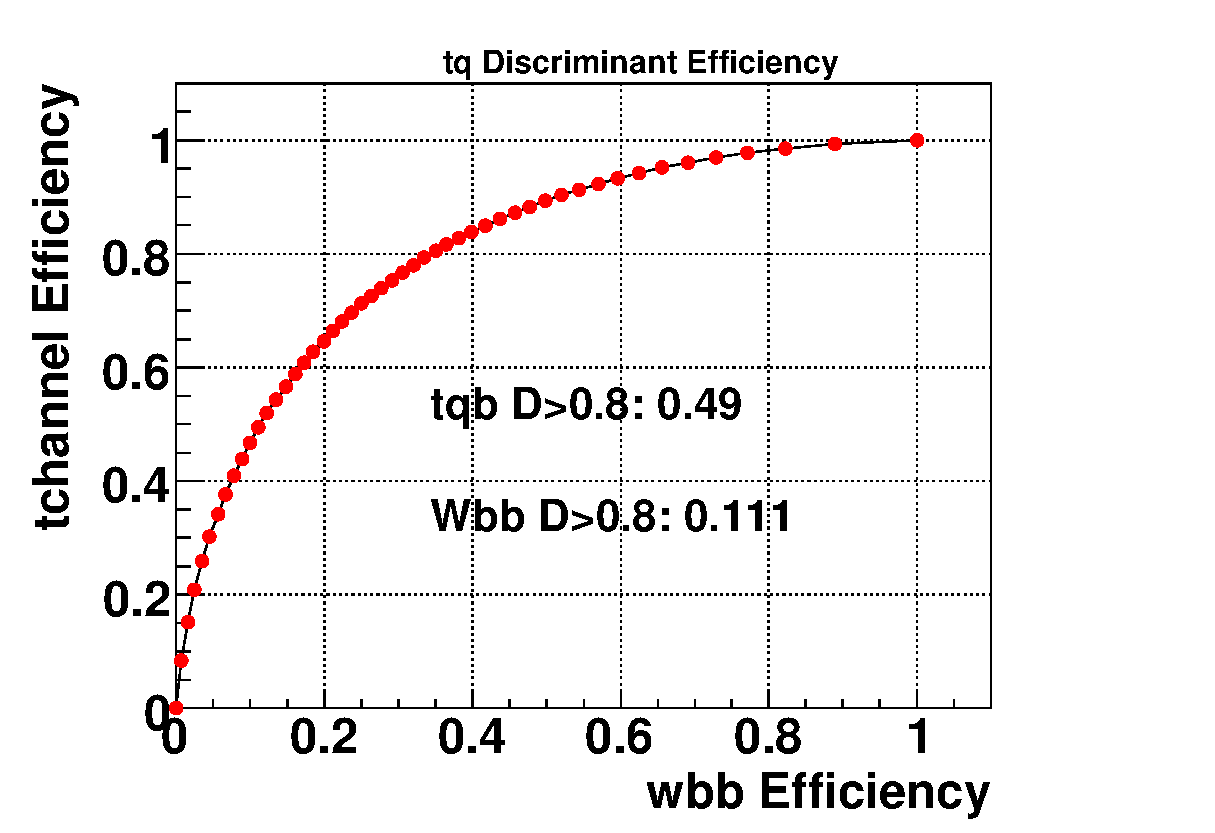
\includegraphics[width=0.49\textwidth]
{eps/MatrixElement/performance/tq_Efficiency__tchannel_wbb}
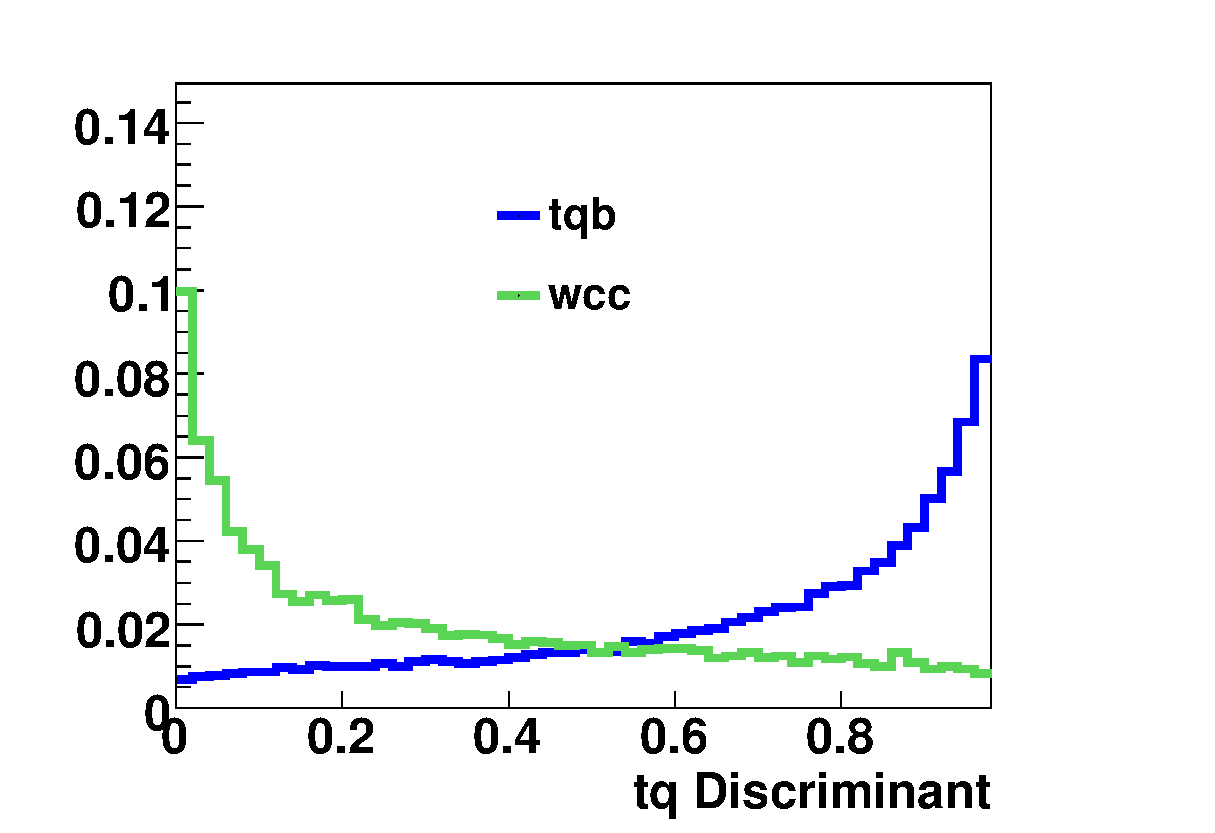
\includegraphics[width=0.49\textwidth]
{eps/MatrixElement/performance/tq_Discriminant__tchannel_wcc}
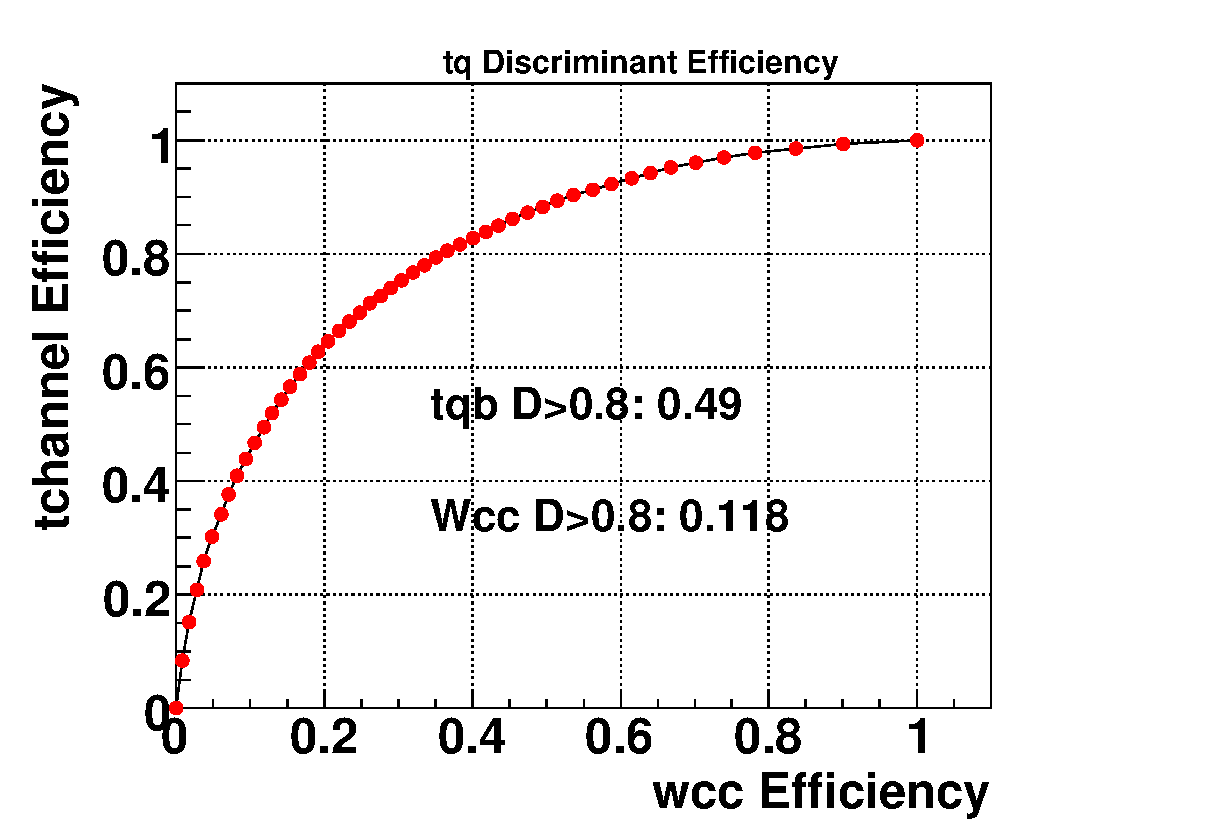
\includegraphics[width=0.49\textwidth]
{eps/MatrixElement/performance/tq_Efficiency__tchannel_wcc}
\caption{Discriminant plots and efficiency curves for:
first row, $tb$ vs. $Wbb$, second row, $tb$ vs. $Wcc$, third row, $tq$
vs. $Wbb$, and fourth row, $tq$ vs. $Wcc$. The numbers in the
efficiency curves (right column) represent the fraction of signal or
background the remains after a discriminant cut of 0.8.}
\label{disc_wbb}
\end{figure}

\begin{figure}[!h!tbp]
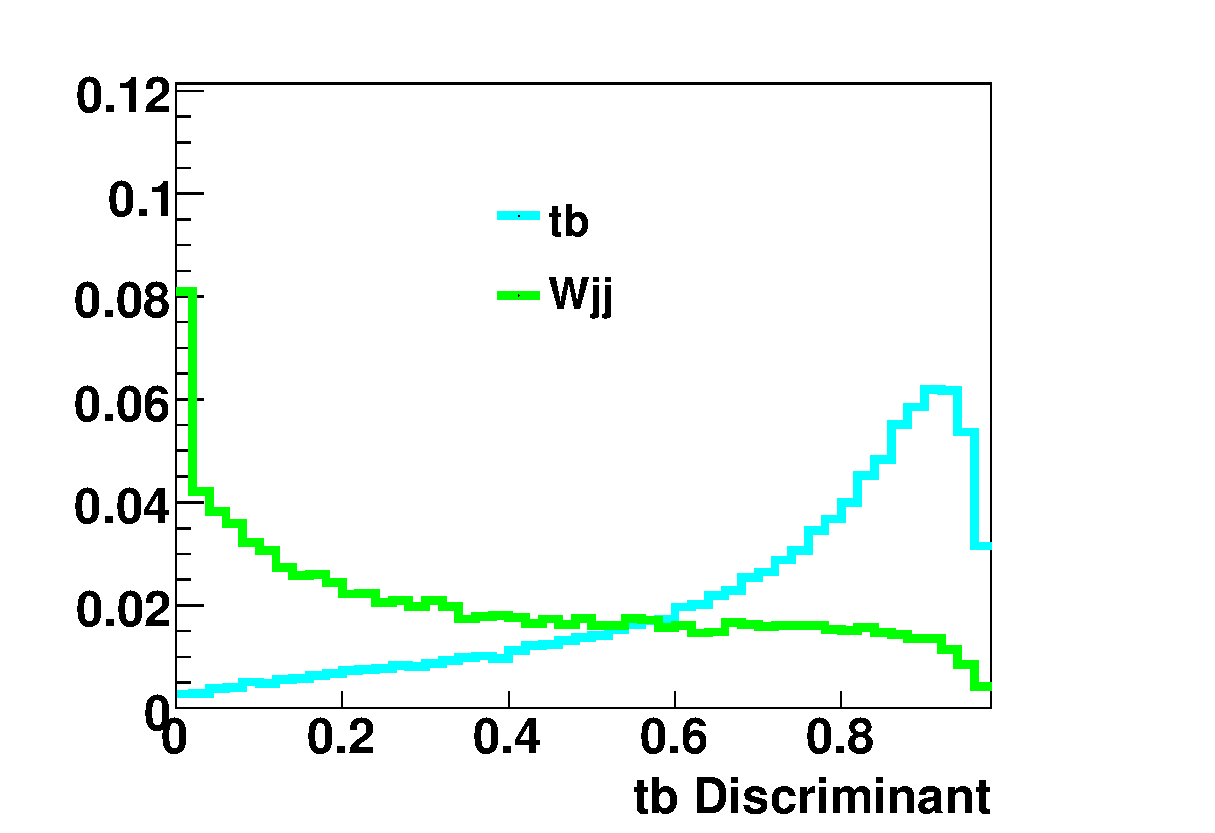
\includegraphics[width=0.49\textwidth]
{eps/MatrixElement/performance/tb_Discriminant__schannel_wjj}
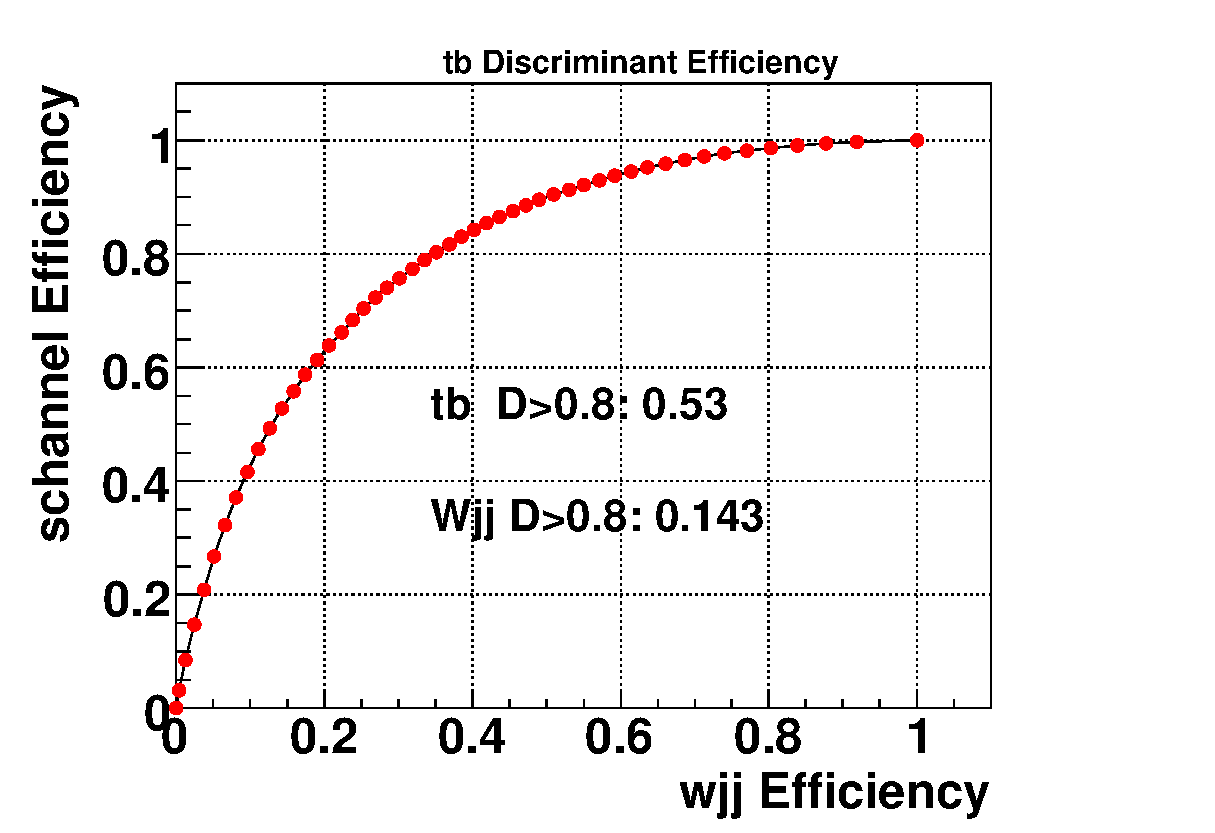
\includegraphics[width=0.49\textwidth]
{eps/MatrixElement/performance/tb_Efficiency__schannel_wjj}
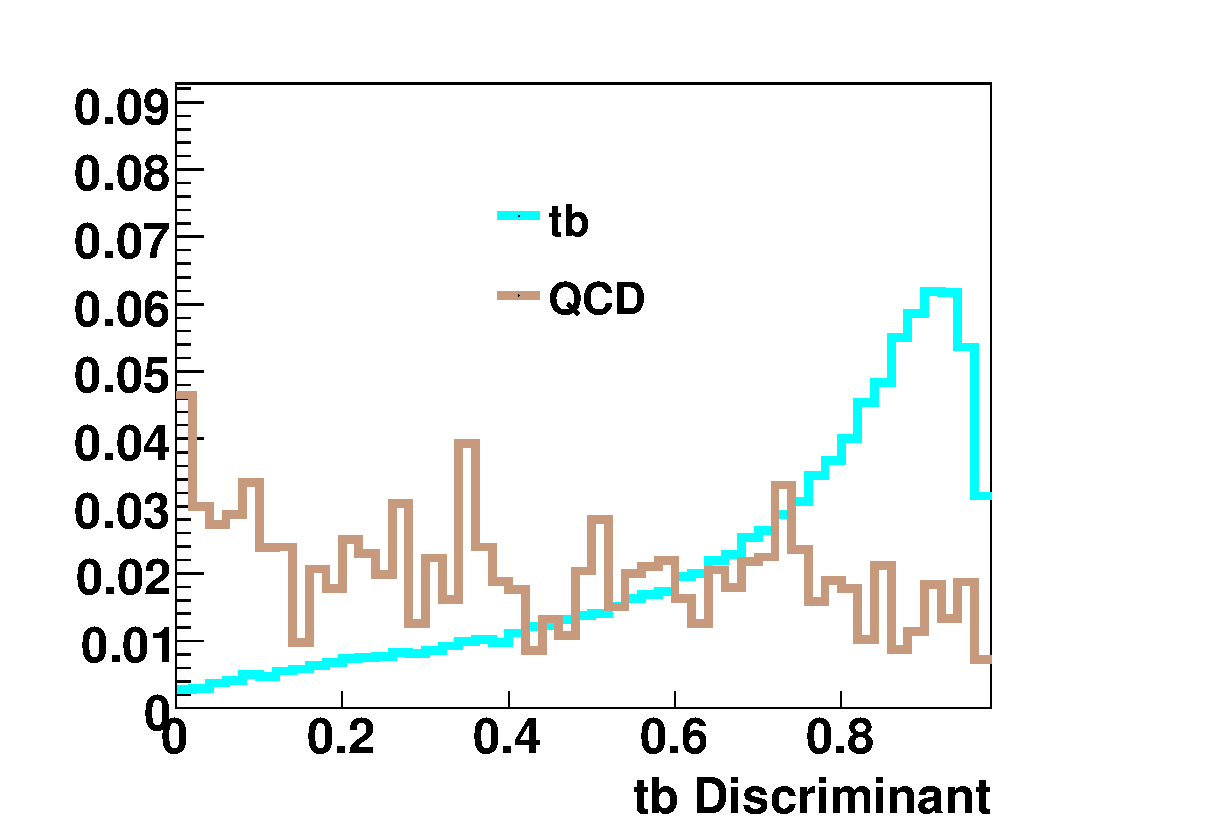
\includegraphics[width=0.49\textwidth]
{eps/MatrixElement/performance/tb_Discriminant__schannel_qcd}
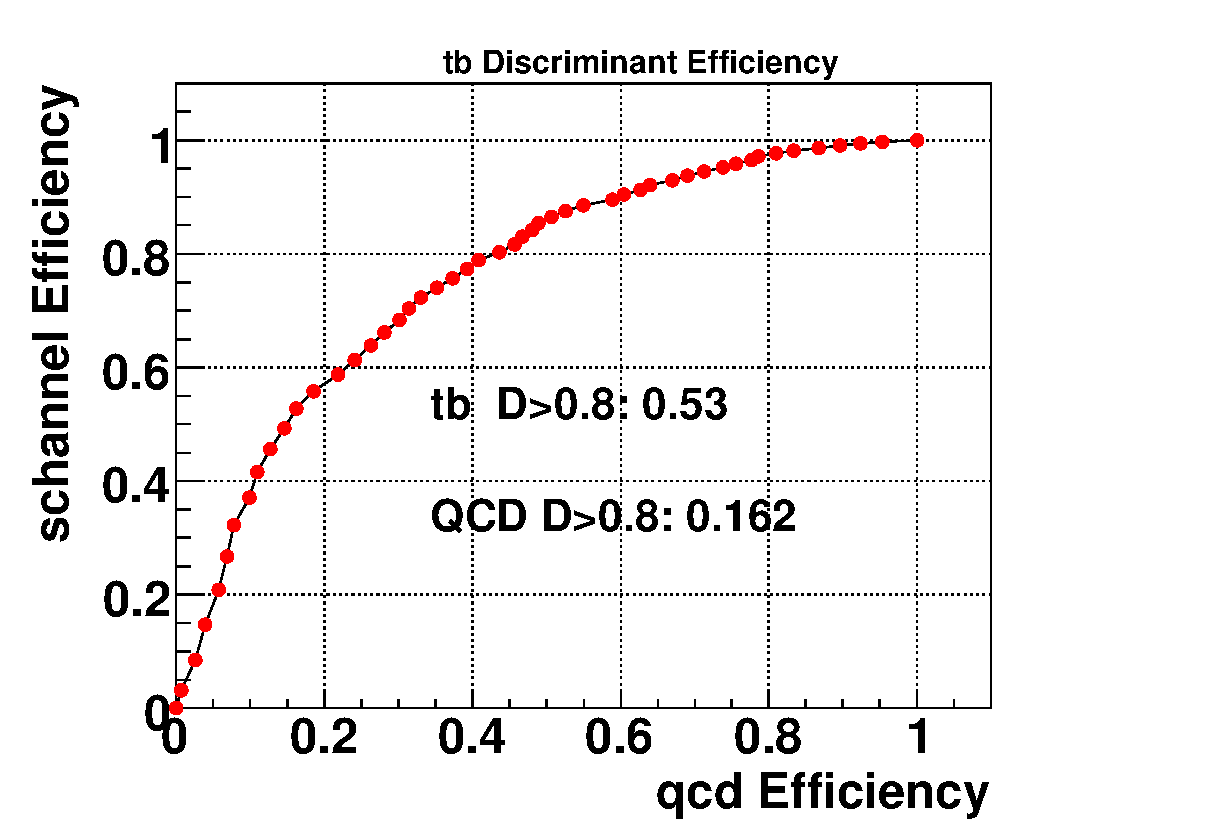
\includegraphics[width=0.49\textwidth]
{eps/MatrixElement/performance/tb_Efficiency__schannel_qcd}
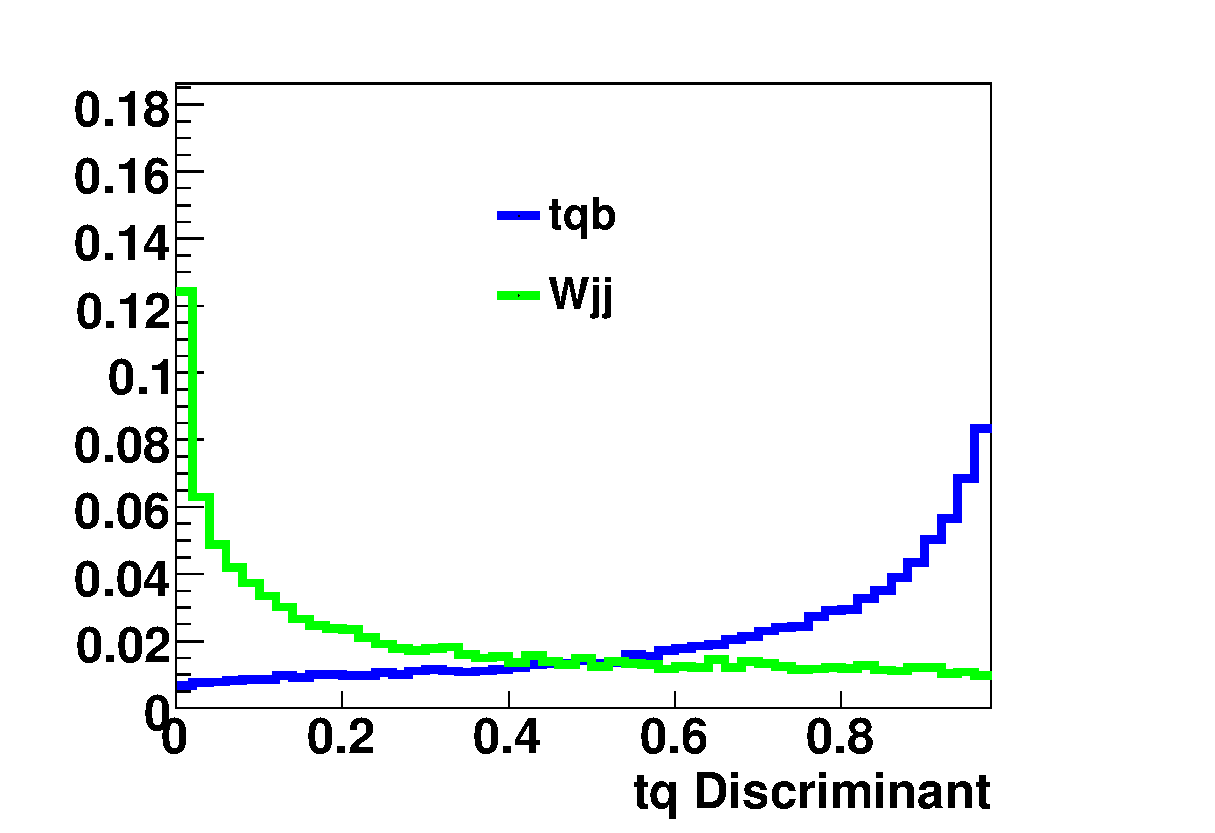
\includegraphics[width=0.49\textwidth]
{eps/MatrixElement/performance/tq_Discriminant__tchannel_wjj}
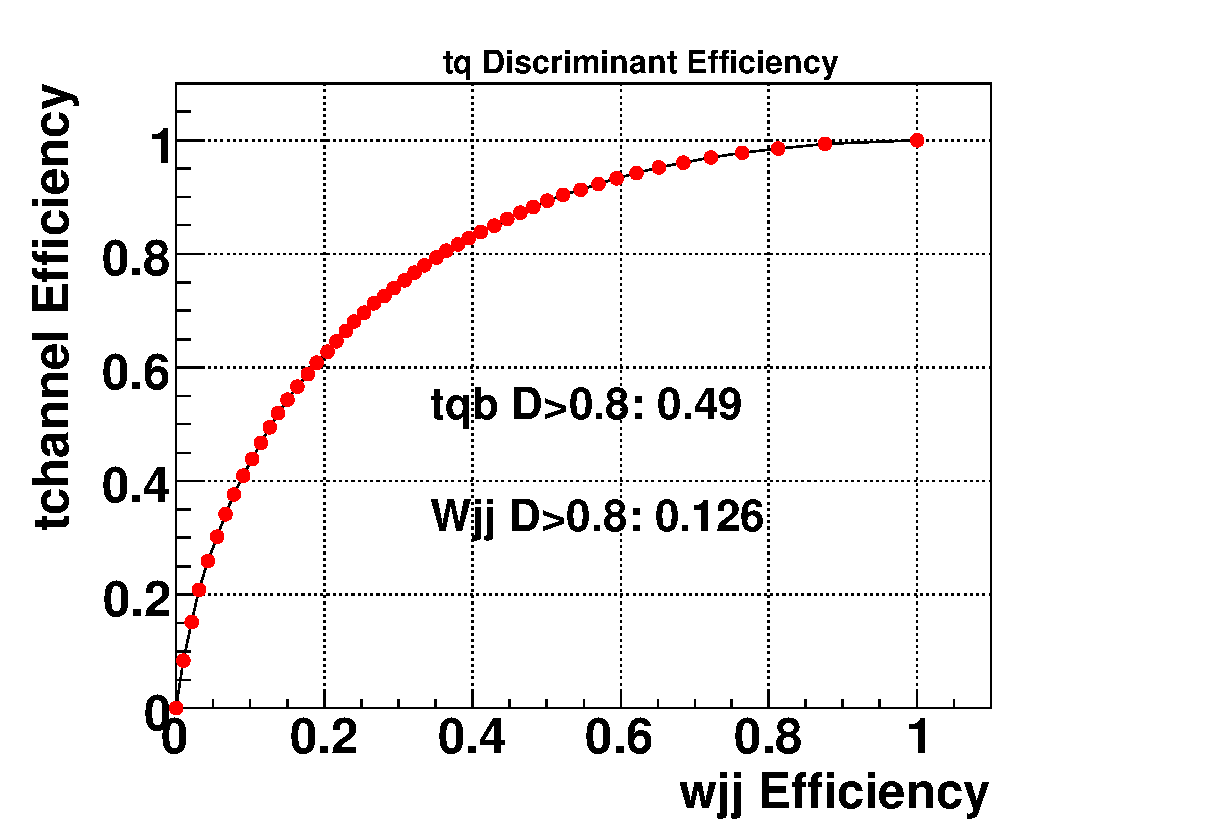
\includegraphics[width=0.49\textwidth]
{eps/MatrixElement/performance/tq_Efficiency__tchannel_wjj}
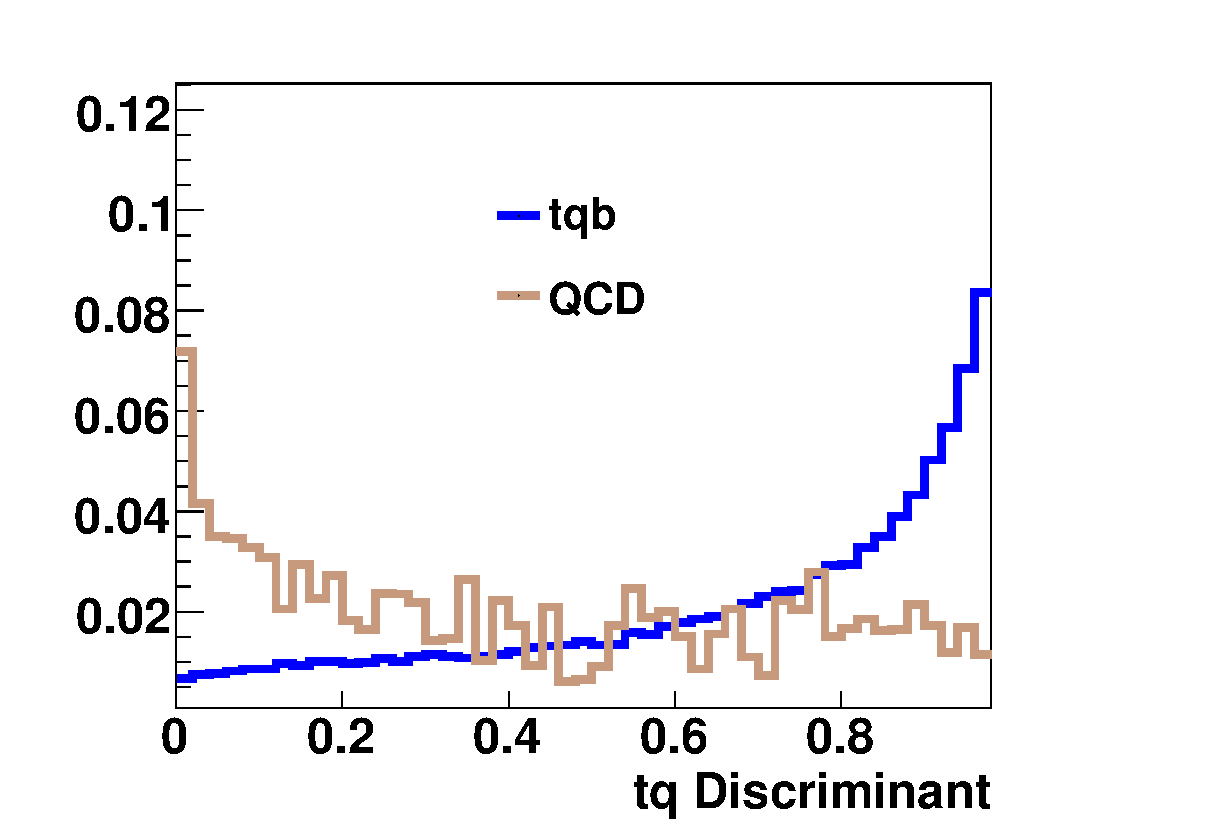
\includegraphics[width=0.49\textwidth]
{eps/MatrixElement/performance/tq_Discriminant__tchannel_qcd}
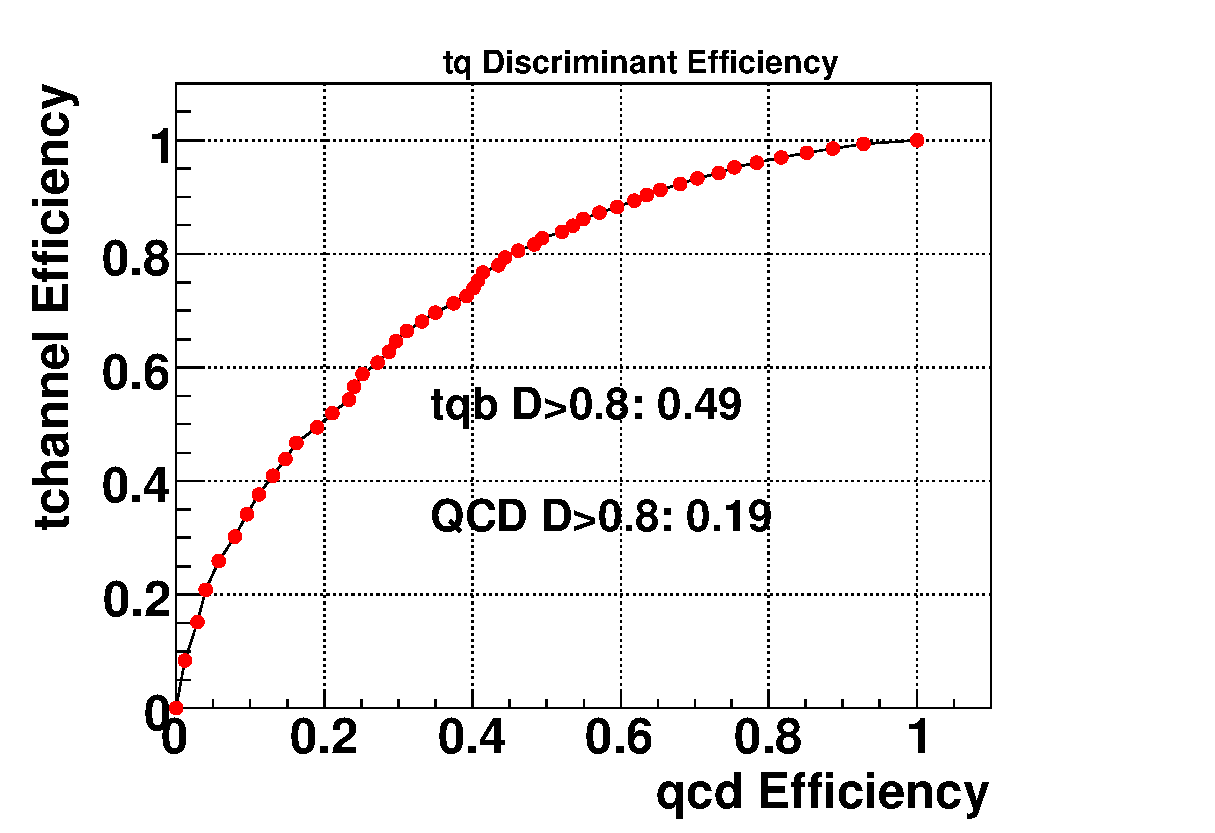
\includegraphics[width=0.49\textwidth]
{eps/MatrixElement/performance/tq_Efficiency__tchannel_qcd}
\caption{Discriminant plots and efficiency curves for:
first row, $tb$ vs. $Wjj$, second row, $tb$ vs. multijets, third row,
$tq$ vs. $Wjj$, and fourth row, $tq$ vs. multijets. The numbers in the
efficiency curves (right column) represent the fraction of signal or
background the remains after a discriminant cut of 0.8.}
\label{disc_wjets}
\end{figure}

\begin{figure}[!h!tbp]
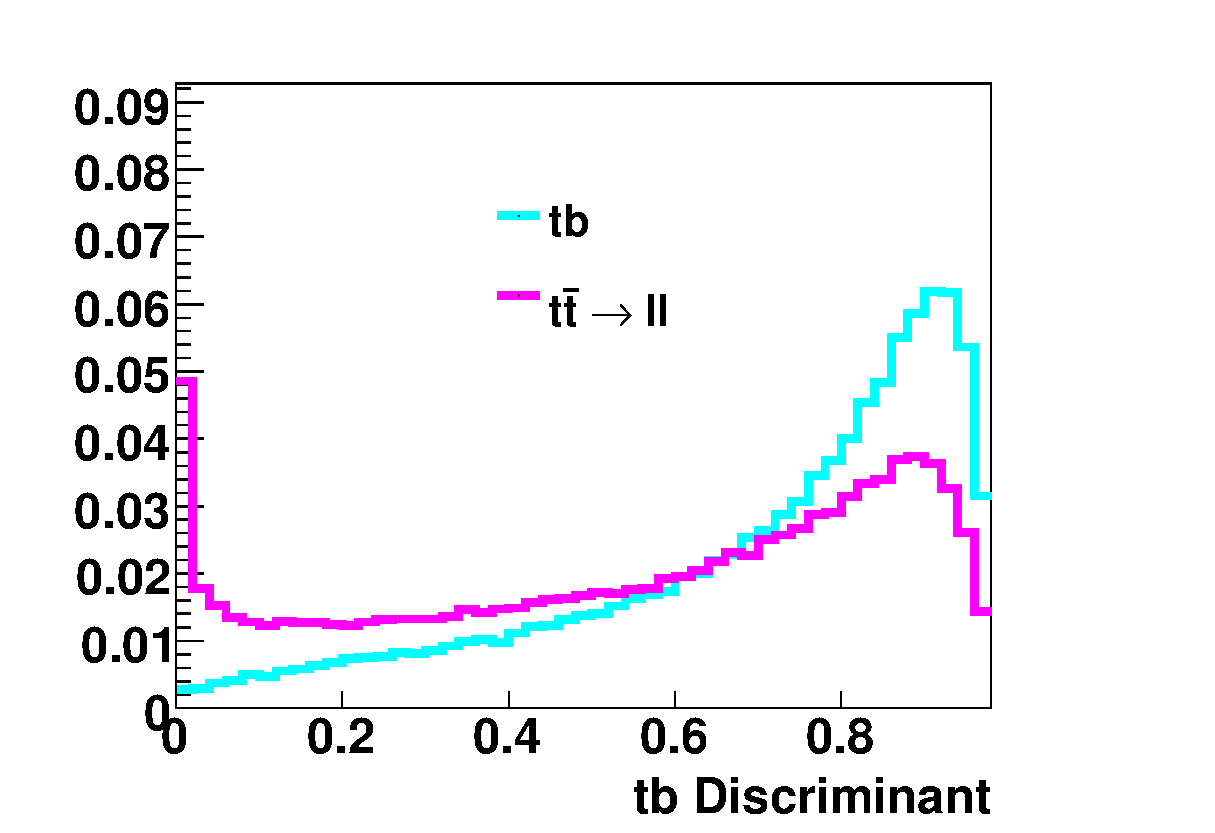
\includegraphics[width=0.49\textwidth]
{eps/MatrixElement/performance/tb_Discriminant__schannel_dilepton}
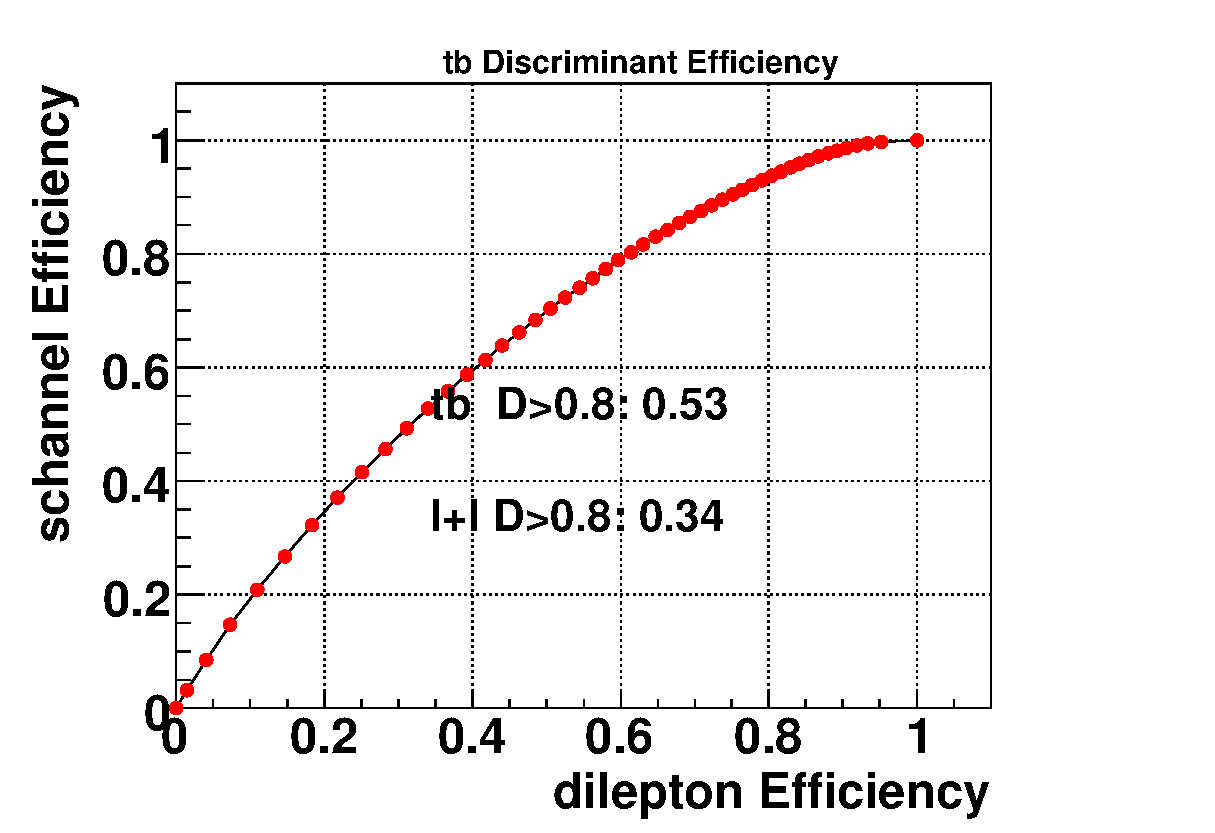
\includegraphics[width=0.49\textwidth]
{eps/MatrixElement/performance/tb_Efficiency__schannel_dilepton}
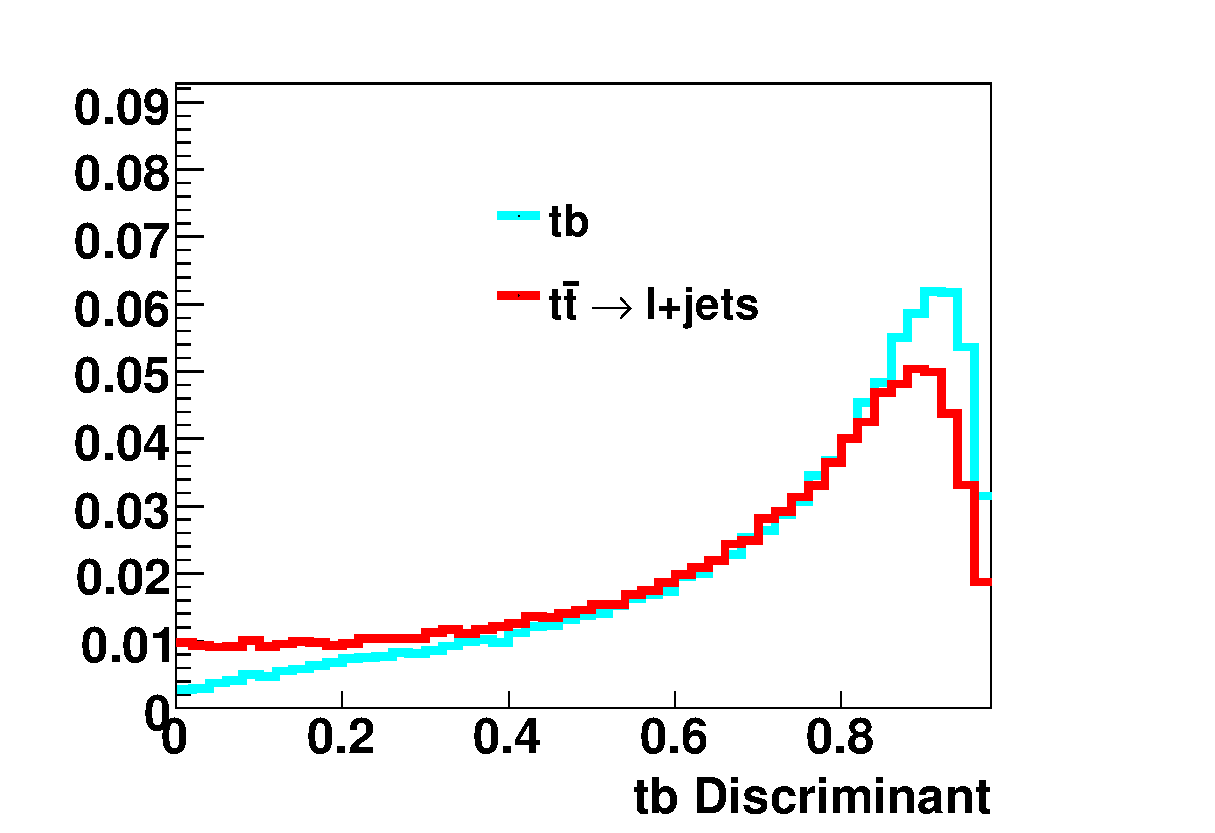
\includegraphics[width=0.49\textwidth]
{eps/MatrixElement/performance/tb_Discriminant__schannel_lepjets}
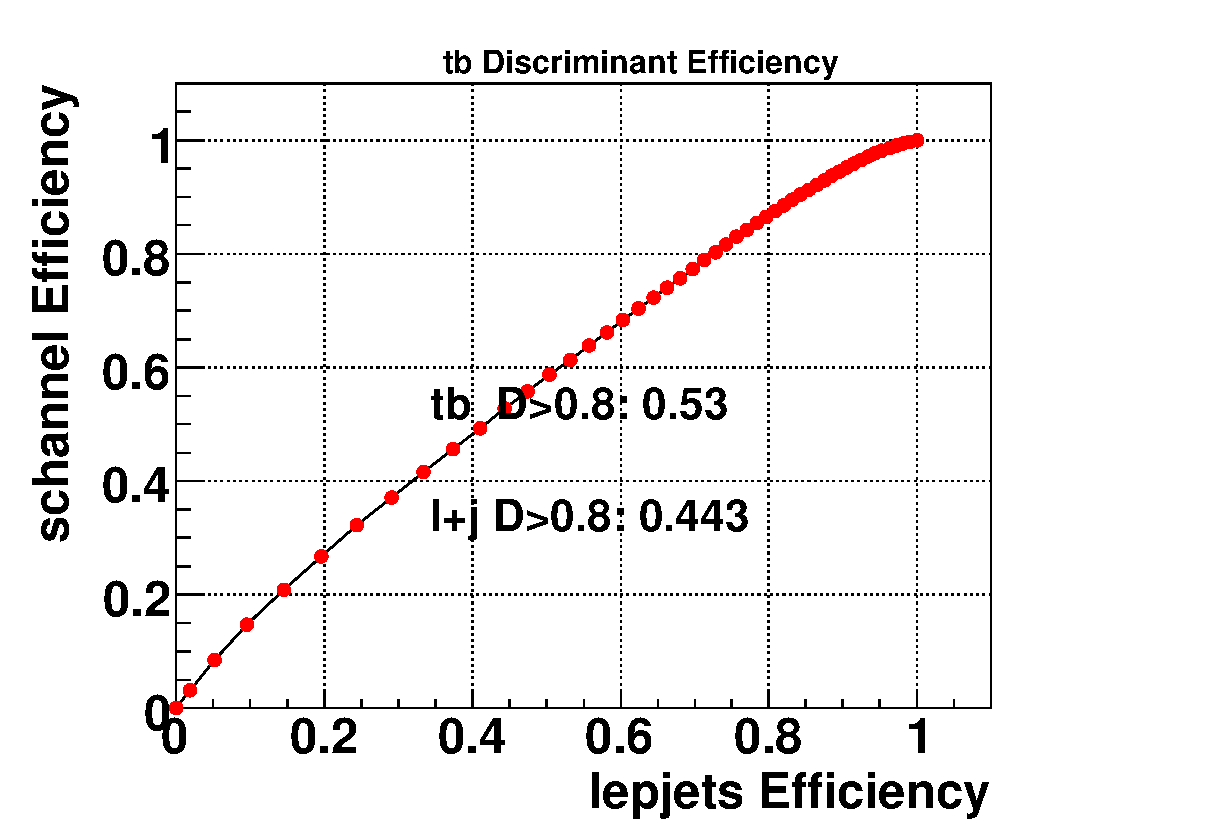
\includegraphics[width=0.49\textwidth]
{eps/MatrixElement/performance/tb_Efficiency__schannel_lepjets}
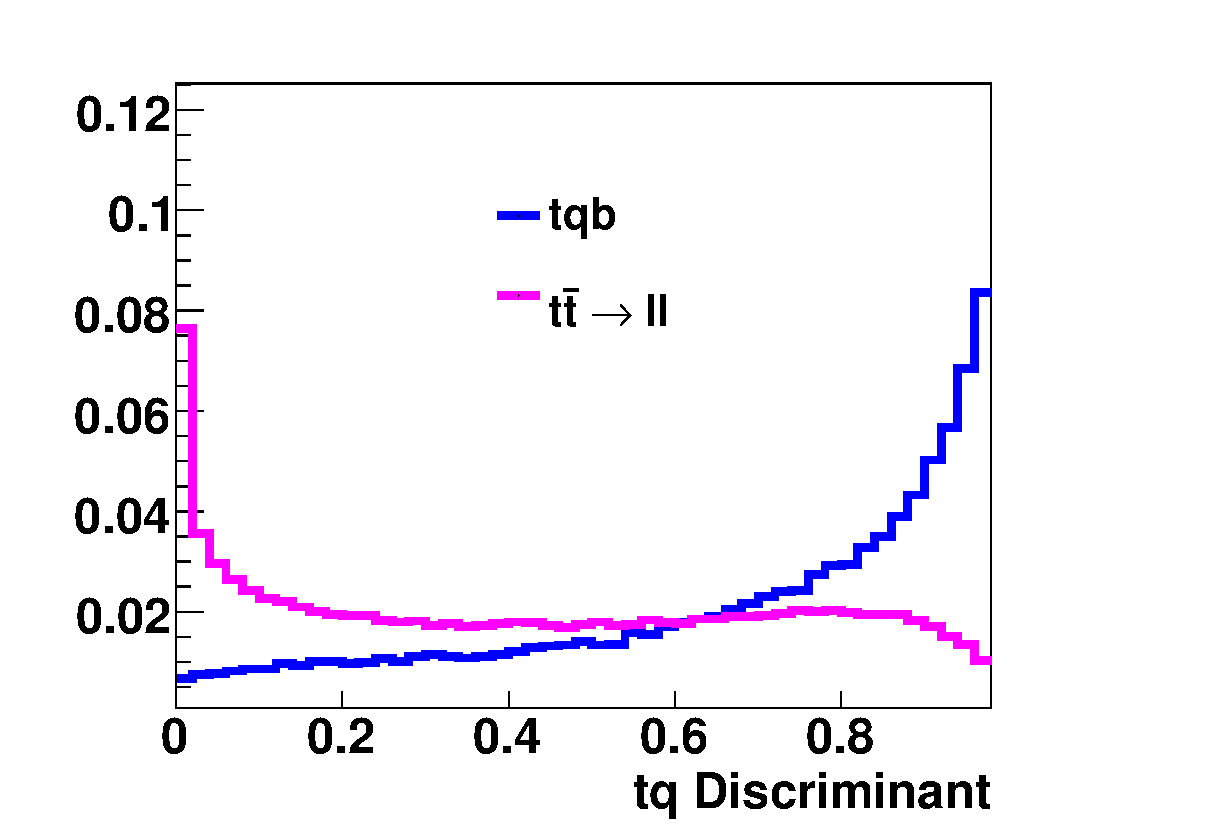
\includegraphics[width=0.49\textwidth]
{eps/MatrixElement/performance/tq_Discriminant__tchannel_dilepton}
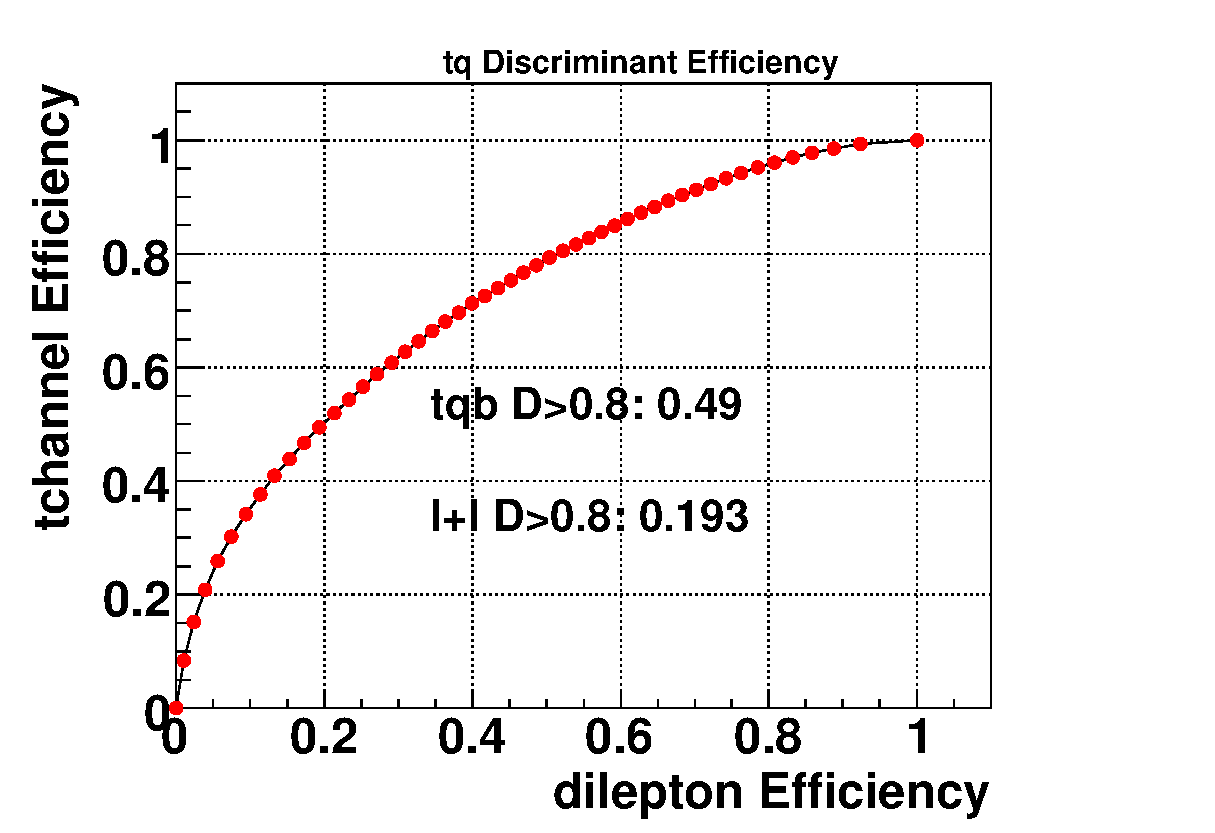
\includegraphics[width=0.49\textwidth]
{eps/MatrixElement/performance/tq_Efficiency__tchannel_dilepton}
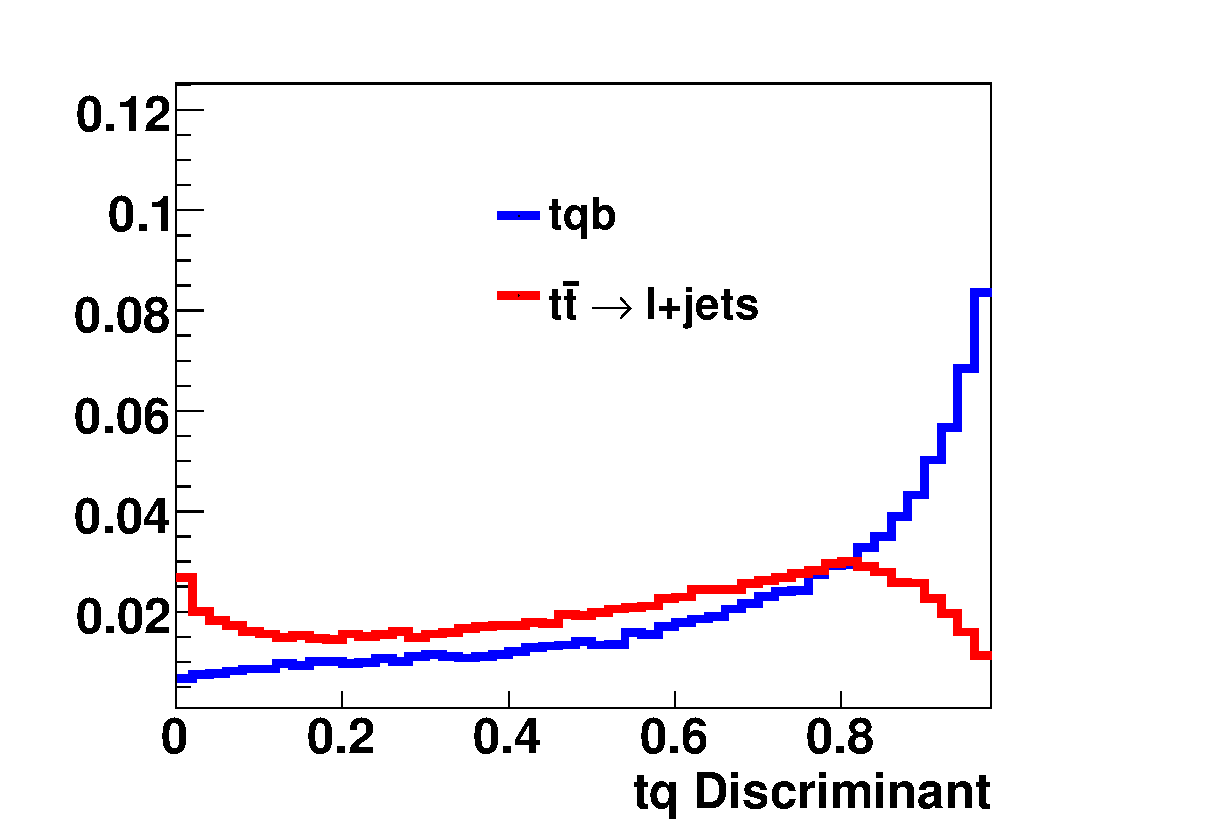
\includegraphics[width=0.49\textwidth]
{eps/MatrixElement/performance/tq_Discriminant__tchannel_lepjets}
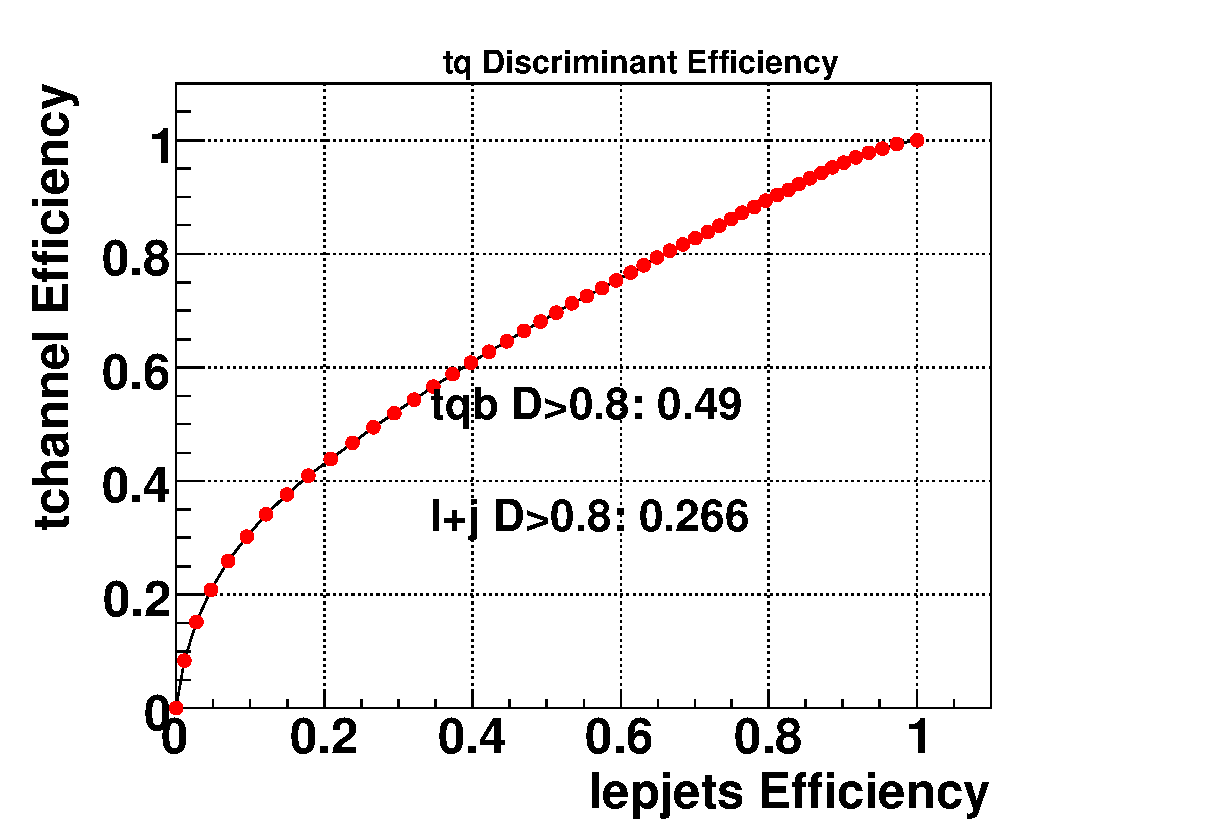
\includegraphics[width=0.49\textwidth]
{eps/MatrixElement/performance/tq_Efficiency__tchannel_lepjets}
\caption{Discriminant plots and efficiency curves for:
first row, $tb$ vs. $\dilepton$, second row, $tb$ vs. $\lepjets$,
third row, $tq$ vs. $\dilepton$, and fourth row, $tq$
vs. $\lepjets$. The numbers in the efficiency curves (right column)
represent the fraction of signal or background the remains after a
discriminant cut of 0.8.}
\label{disc_ttbar}
\end{figure}

\subsection{Two-Dimensional Discriminants}

This analysis uses a two-dimensional (2D) discriminant as the final output where one axis is the $s$-channel discriminant and the other axis is the $t$-channel discriminant value for the event. The 2D discriminant is more powerful than either 1D
projection because it selects events with both $s$ and $t$-channel
characteristics, which helps to further reduce the $W$+jets and
$\ttbar$ background which may have either characteristic but not
necessarily both. Figures~\ref{wbbwccwjj} and \ref{qcdtt} show the 2D discriminants
for single top quark signals and for all the backgrounds. The
plots are normalized to unit volume.

\clearpage

\begin{figure}[!h!tbp]
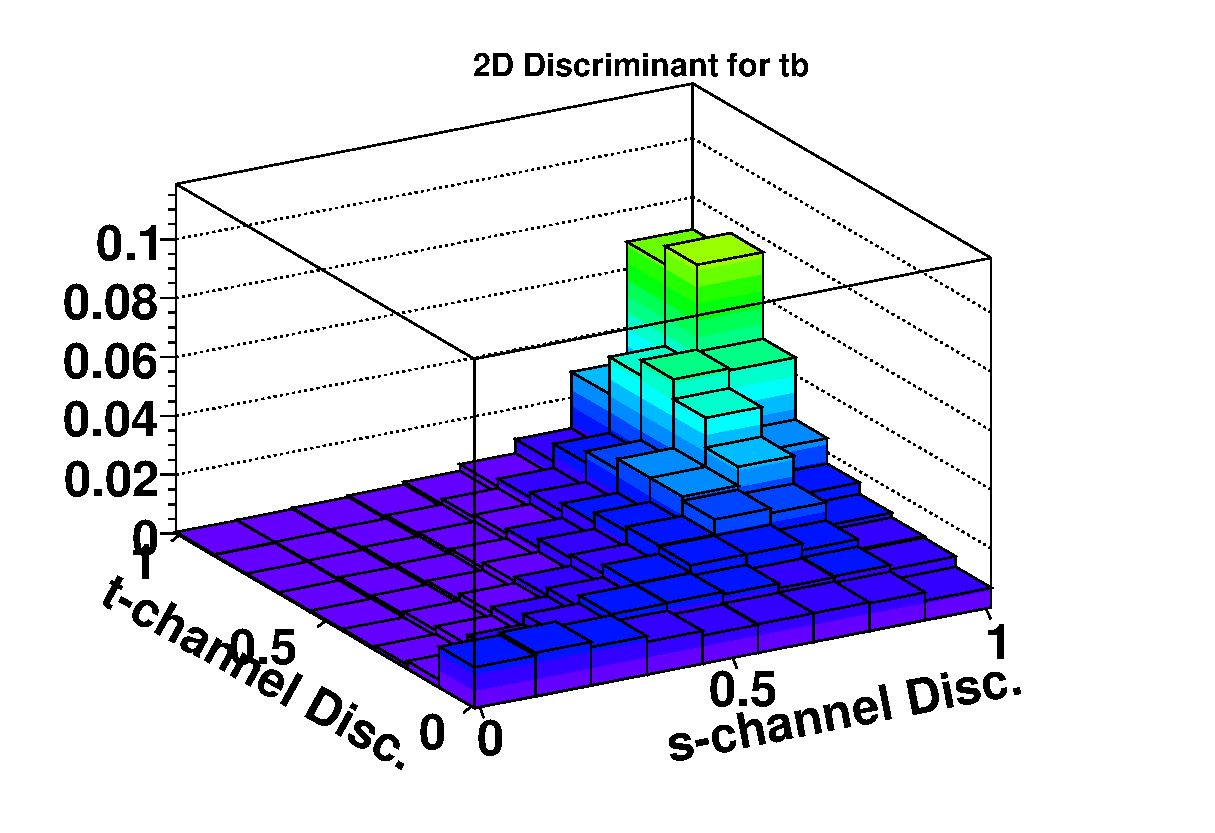
\includegraphics[width=0.49\textwidth]
{eps/MatrixElement/performance/2D-Discriminant_schannel}
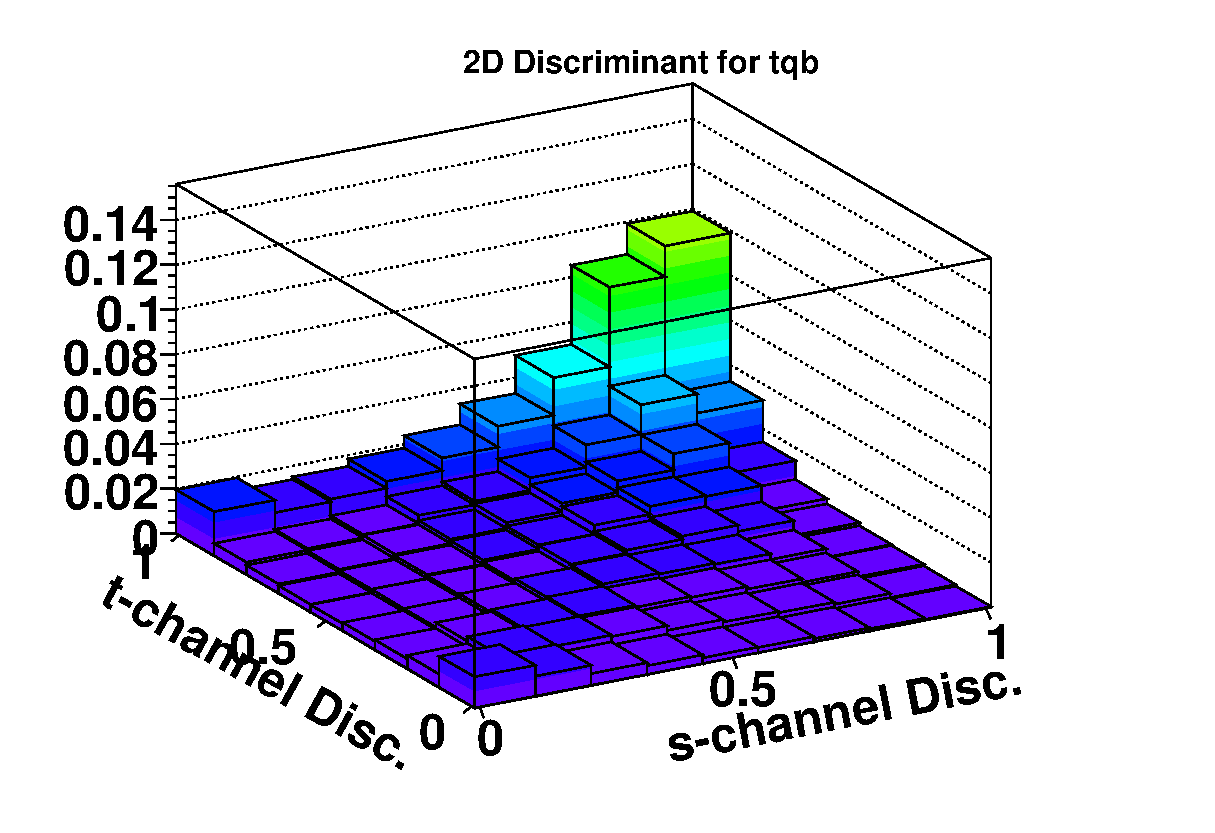
\includegraphics[width=0.49\textwidth]
{eps/MatrixElement/performance/2D-Discriminant_tchannel}
\vspace{-0.1in}
\caption{2D-discriminant templates for: left, $tb$, and
right, $tqb$ Monte Carlo events.}
\label{tbtqb}
\end{figure}

\begin{figure}[!h!tbp]
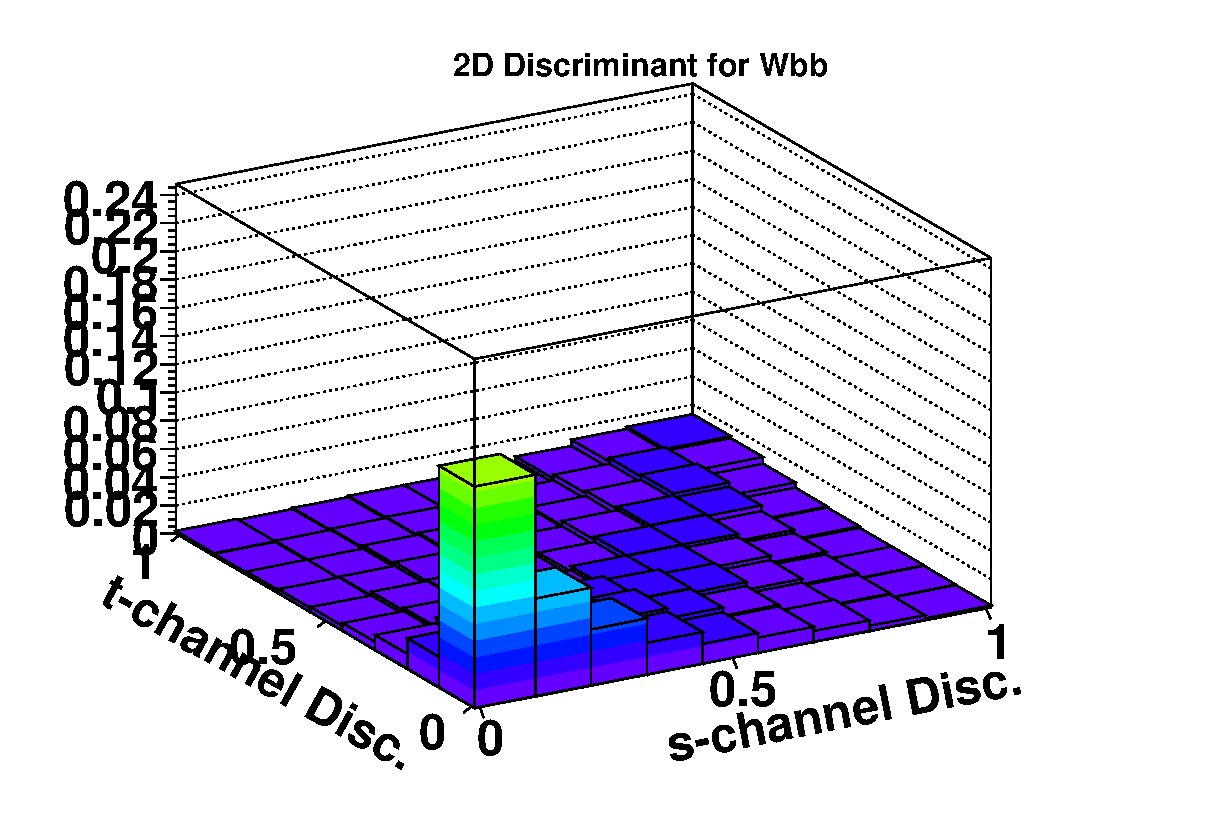
\includegraphics[width=0.49\textwidth]
{eps/MatrixElement/performance/2D-Discriminant_wbb}
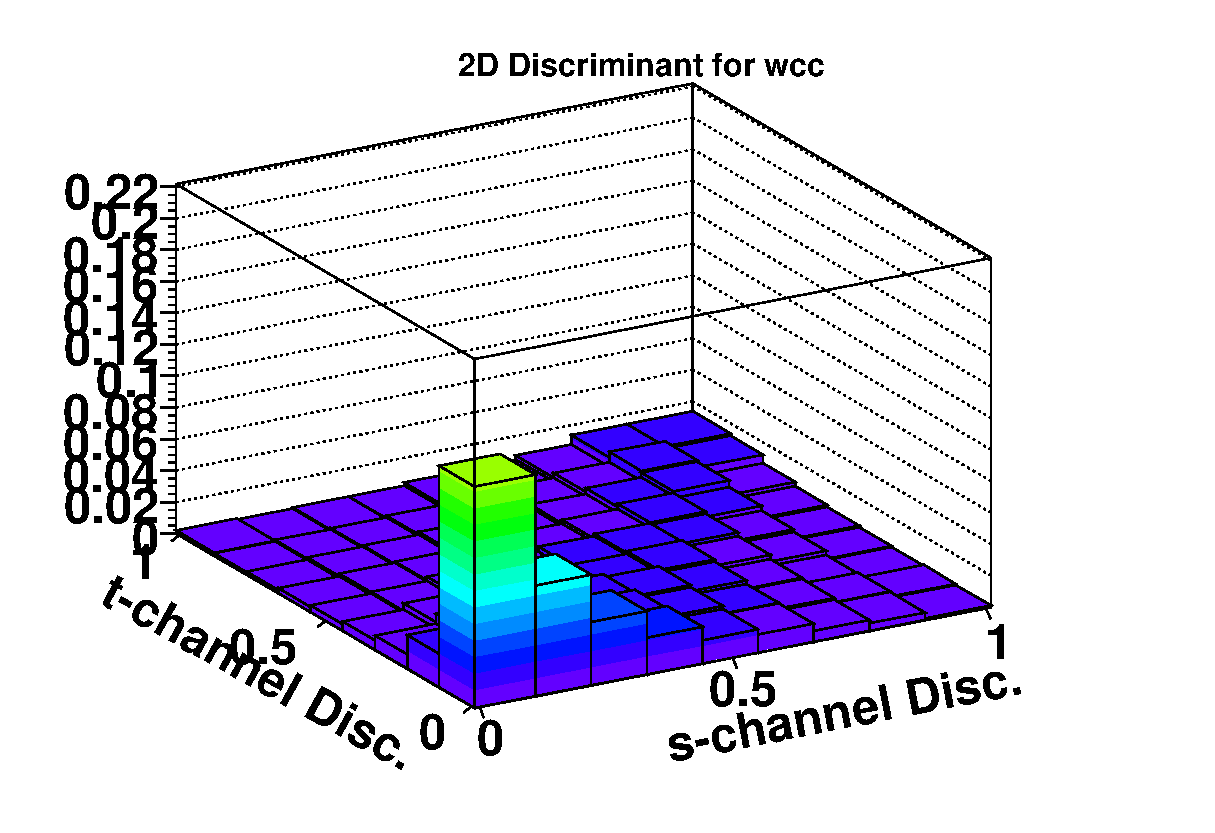
\includegraphics[width=0.49\textwidth]
{eps/MatrixElement/performance/2D-Discriminant_wcc}
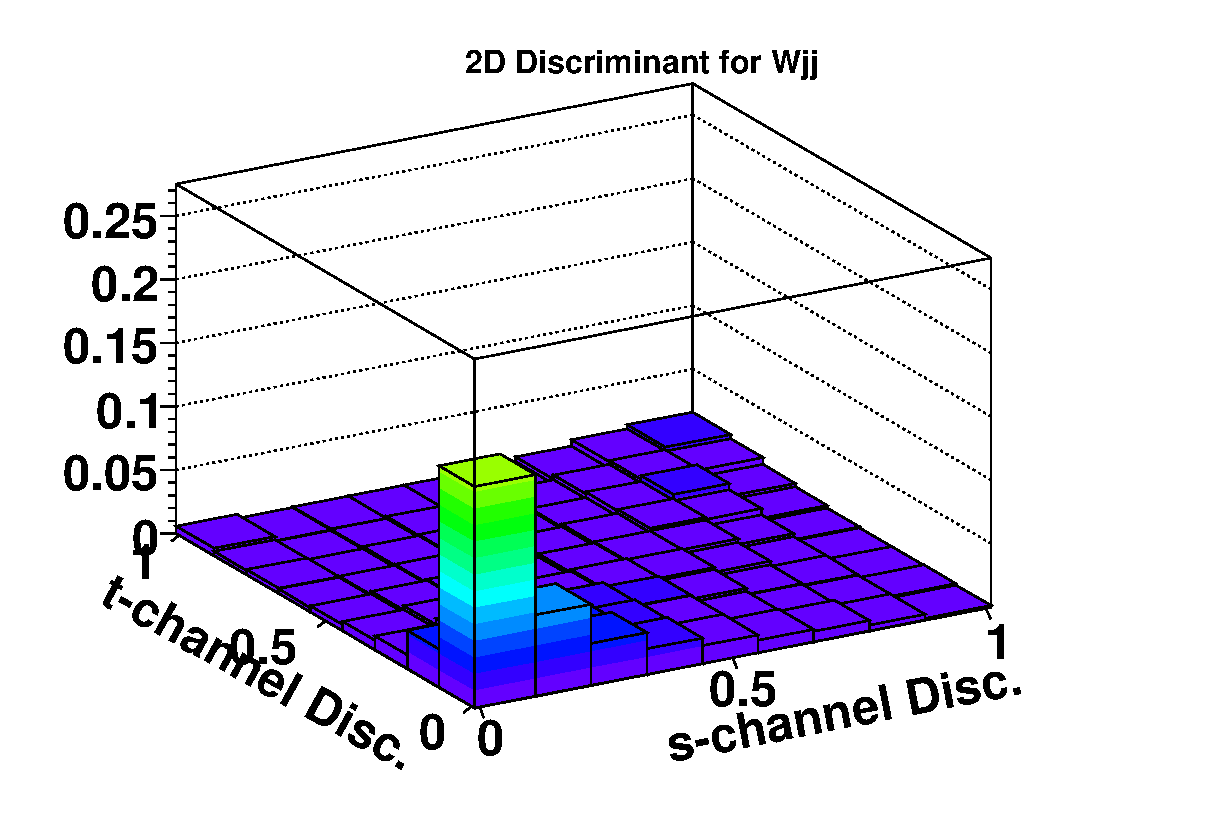
\includegraphics[width=0.49\textwidth]
{eps/MatrixElement/performance/2D-Discriminant_wjj}
\vspace{-0.1in}
\caption{2D-discriminant templates for: left,
$Wbb$, middle, $Wcc$, and right, $Wjj$ Monte Carlo events.}
\label{wbbwccwjj}
\end{figure}

\begin{figure}[!h!tbp]
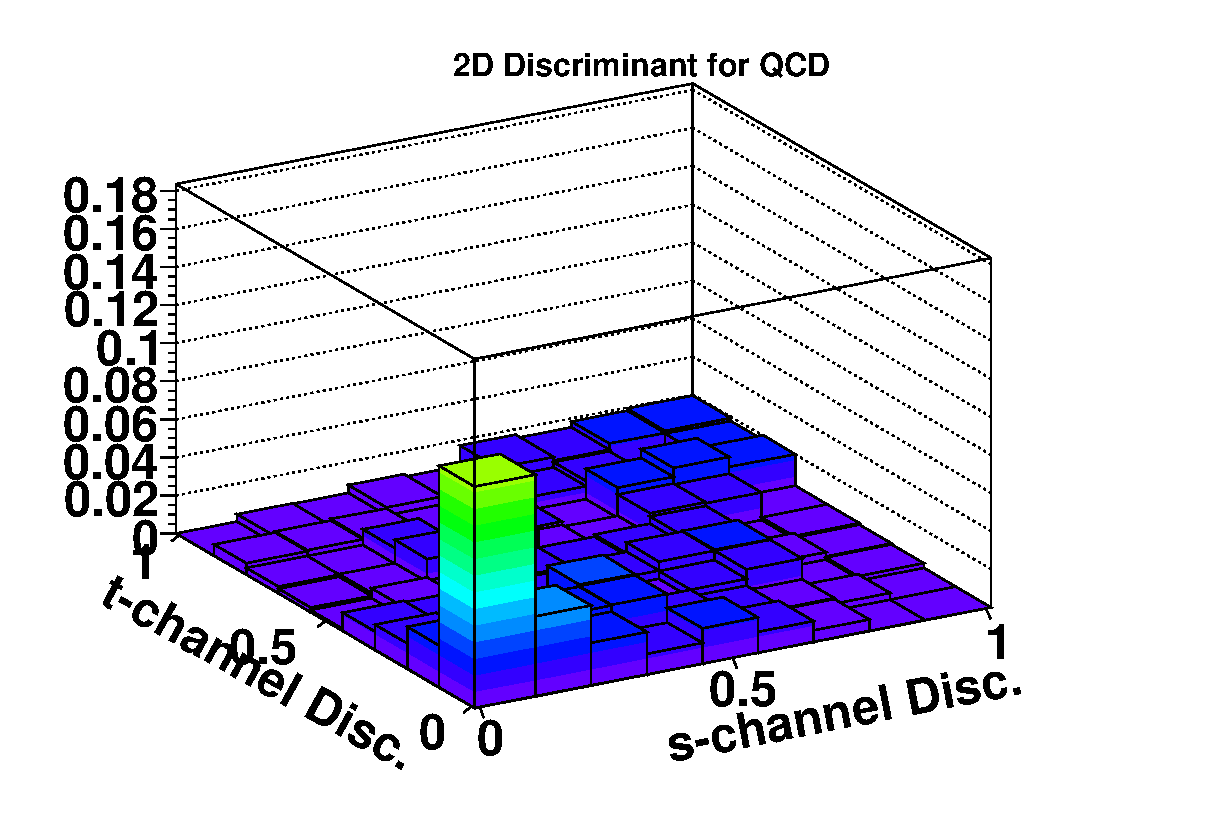
\includegraphics[width=0.49\textwidth]
{eps/MatrixElement/performance/2D-Discriminant_qcd}
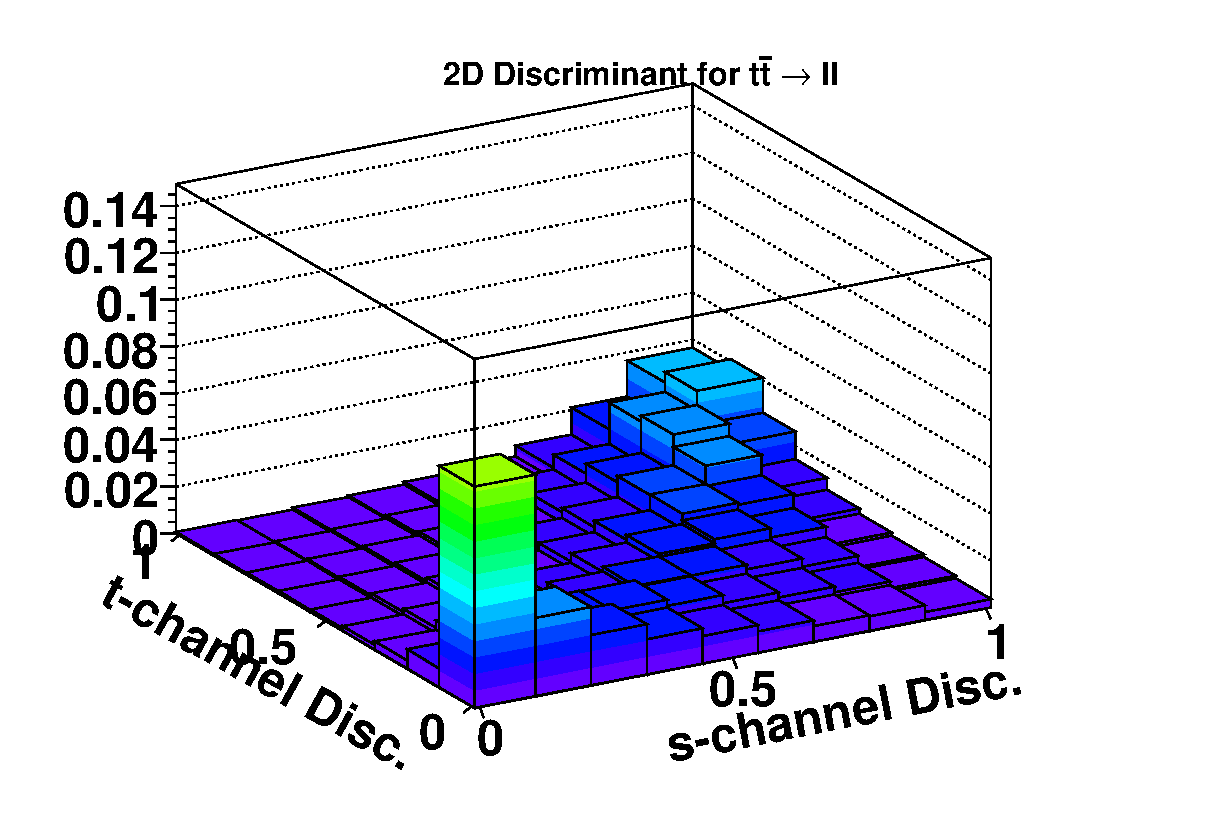
\includegraphics[width=0.49\textwidth]
{eps/MatrixElement/performance/2D-Discriminant_dilepton}
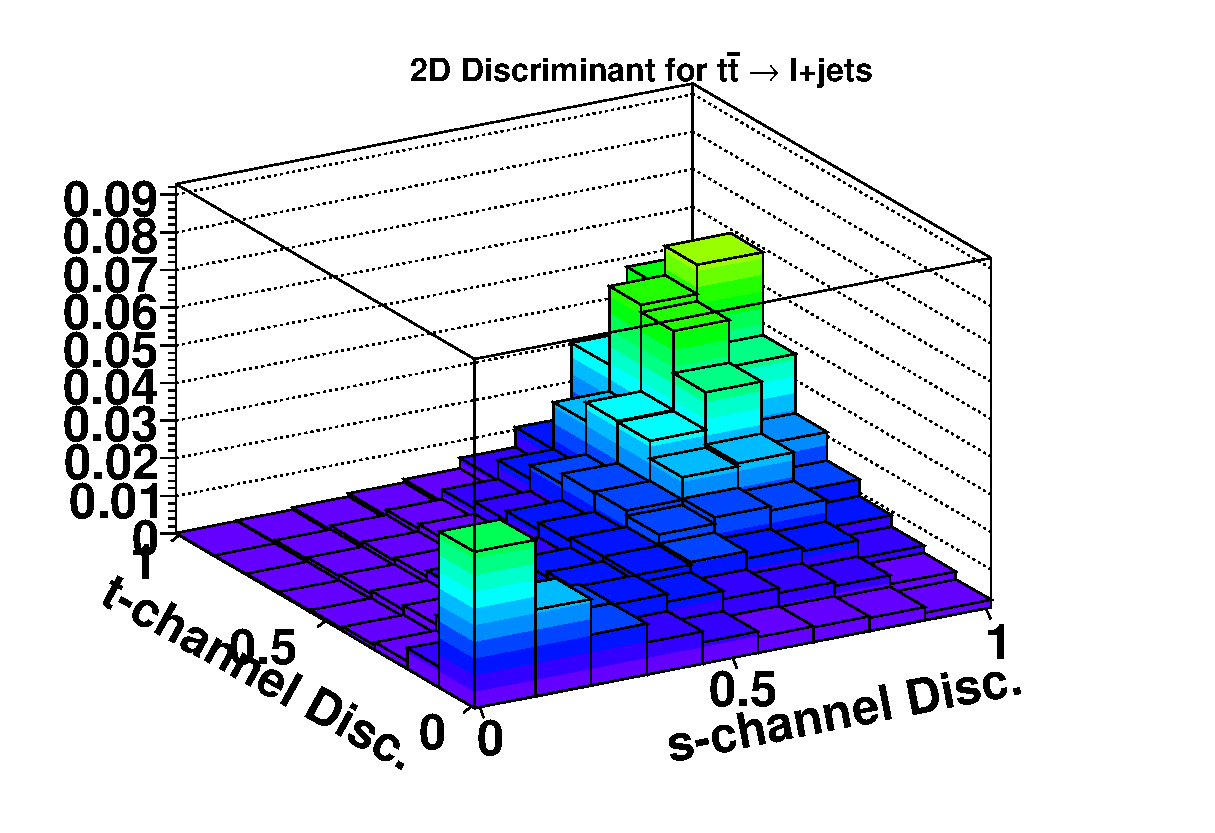
\includegraphics[width=0.49\textwidth]
{eps/MatrixElement/performance/2D-Discriminant_lepjets}
\vspace{-0.1in}
\caption{2D-discriminant templates for: left,
multijets events, middle, $\dilepton$, and right, $\lepjets$ Monte
Carlo events.}
\label{qcdtt}
\end{figure}



\section{Cross-Check Samples}
\label{crosscheck}

Before a measurement of the single top quark cross section is made, the output of the matrix element analysis is compared between data and background in a region where the signal content is negligible. If the agreement between data and background is good in this sample, there is more confidence that the background is well-modeled in the signal region. In this analysis two background-dominated control
samples are defined, and a comparison between the 1D discriminants in
data and the background model is performed.

These two control samples are selected by applying the nominal event
selection, and requiring in addition cut on the total transverse energy $H_{T}$ defined as

\begin{equation}
H_{T} = p^{\rm{lepton}}_{T} + \rm{M}E_{T} + \sum_{\rm{jets}} p^{jet}_{T}
\end{equation}

The first sample selects events with $H_T<175$~GeV and the second sample selects events with $H_T>300$~GeV,
respectively. The control samples defined with $H_{T}<175$~GeV is referred to as the ``soft $W$+jets'' sample and the sample with $H_{T}>300$~GeV is referred to as the ``hard $W$+jets'' sample. In the case of three-jet events, the ``hard $W$+jets'' sample also contains a
significant fraction of $\ttbar$.

The ``soft $W$+jets'' sample selects low momentum $W$+jets and
multijets events and almost no top-quark events.
Figures~\ref{wjets-cross-2jet} and \ref{wjets-cross-3jet} compare the
$s$-channel and $t$-channel discriminants between data and the background model for
events with two and three jets respectively.

The ``hard $W$+jets'' sample selects mainly $\ttbar$ and high momentum
$W$+jets events. Figures~\ref{ttbar-cross-2jet} and
\ref{ttbar-cross-3jet} compare the $s$-channel and $t$-channel discriminants between
data and the background model for events with two and three jets.

\clearpage
\begin{figure}[!h!tbp]
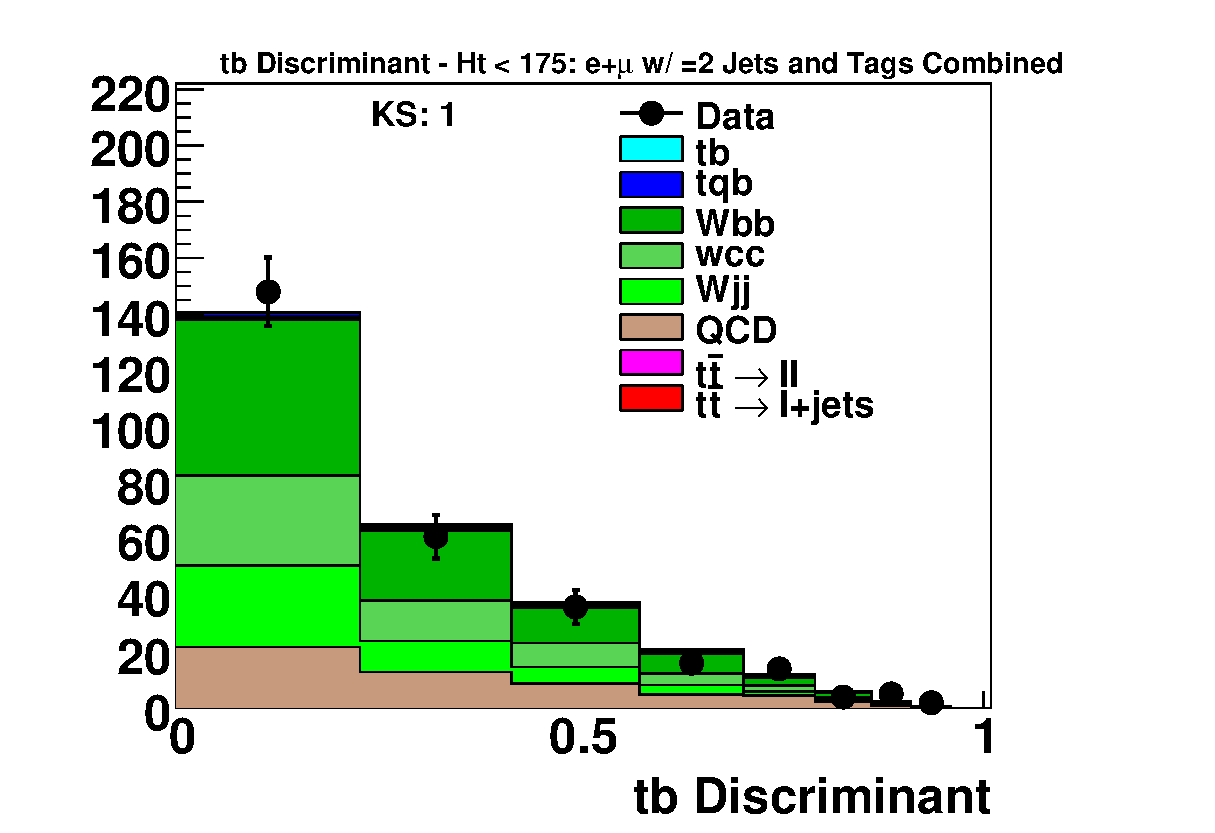
\includegraphics[width=0.49\textwidth]
{eps/MatrixElement/cross_check/combined/2jet/Wjets_tb_Discriminant}
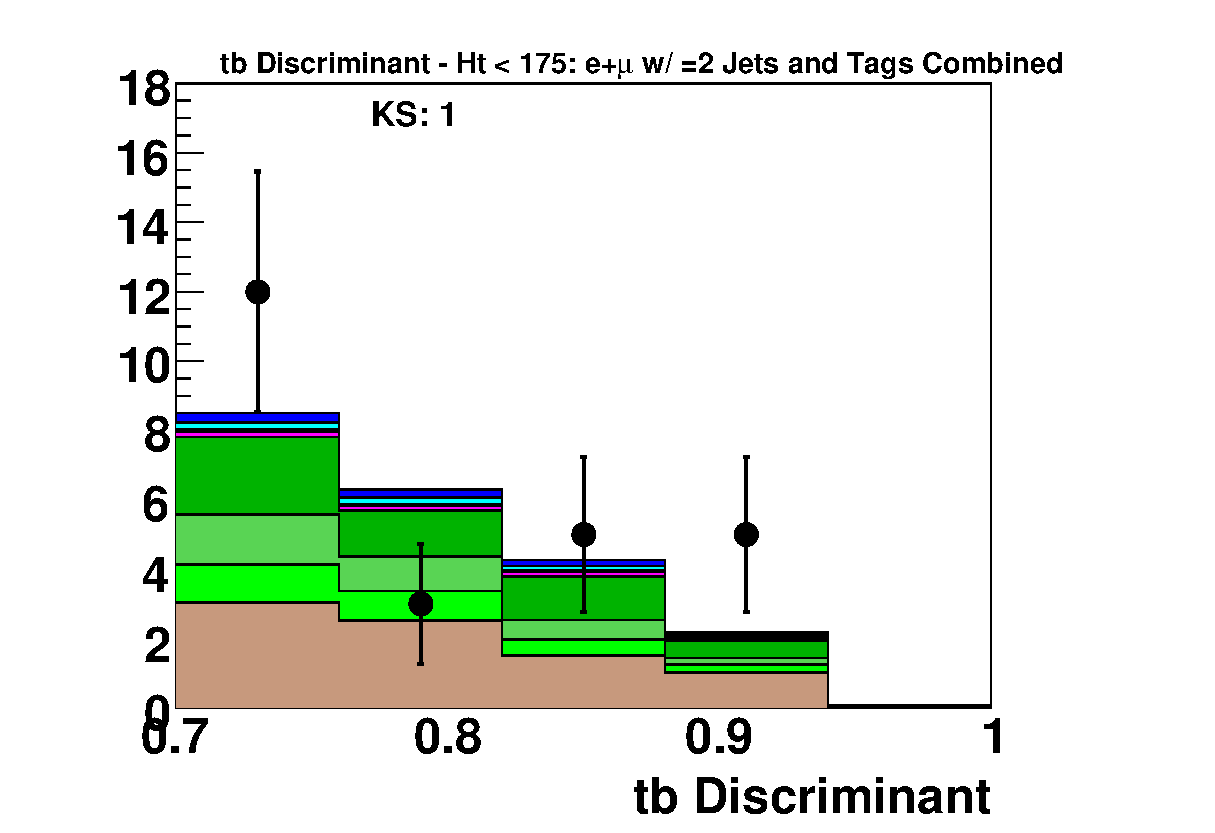
\includegraphics[width=0.49\textwidth]
{eps/MatrixElement/cross_check/combined/2jet/Wjets_tb_Discriminant_Zoom}
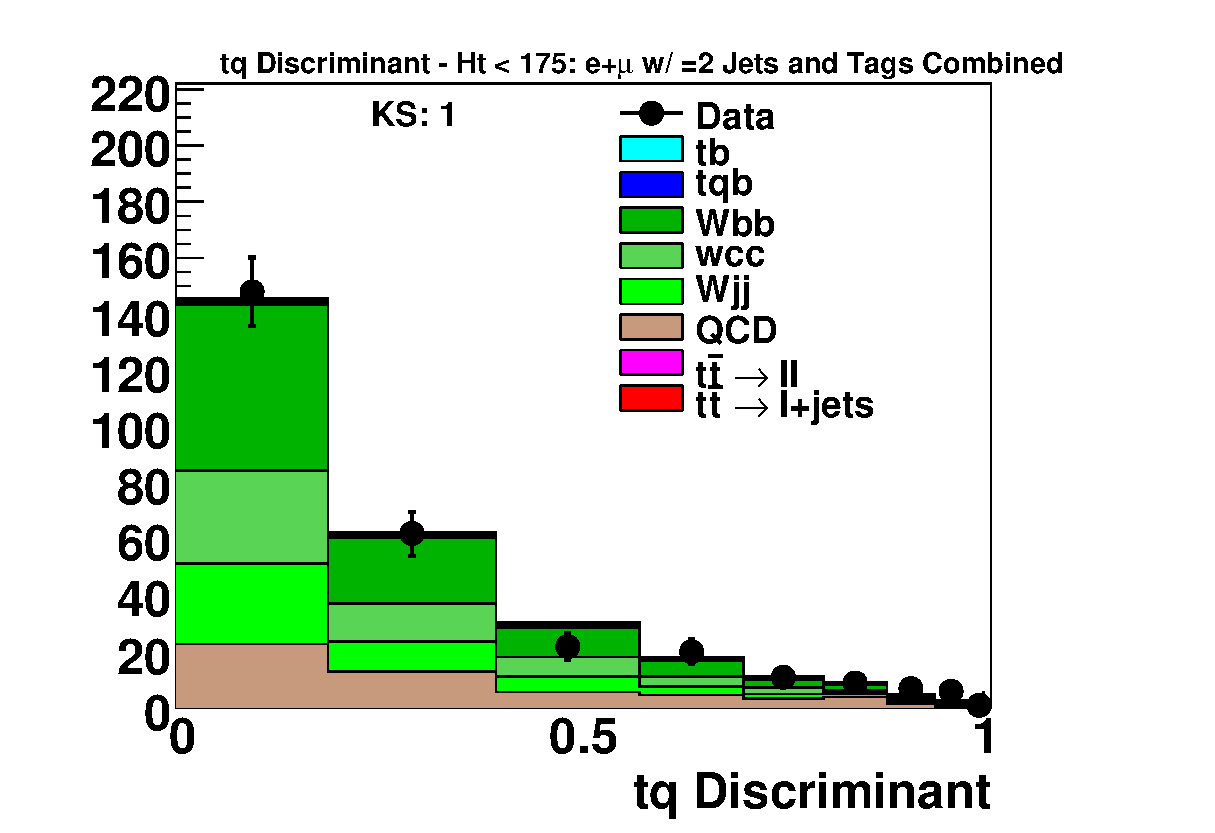
\includegraphics[width=0.49\textwidth]
{eps/MatrixElement/cross_check/combined/2jet/Wjets_tq_Discriminant}
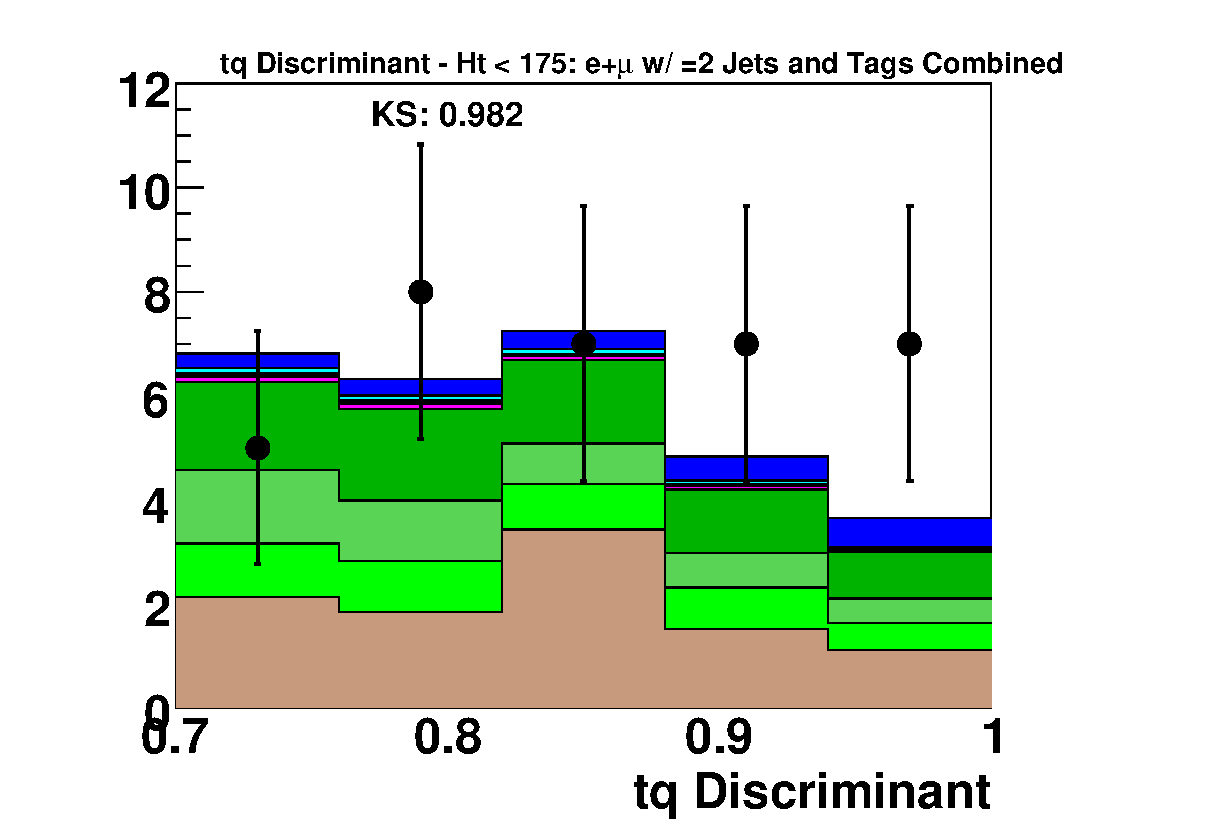
\includegraphics[width=0.49\textwidth]
{eps/MatrixElement/cross_check/combined/2jet/Wjets_tq_Discriminant_Zoom}
\vspace{-0.1in}
\caption{``Soft $W$+jets'' cross-check plots in two-jet
events for the $tb$ discriminant (upper row) and the $tq$ discriminant
(lower row). The left column shows the full discriminant region while
the right column shows the high discriminant region above 0.7.}
\label{wjets-cross-2jet}
\end{figure}

\clearpage
\begin{figure}[!h!tbp]
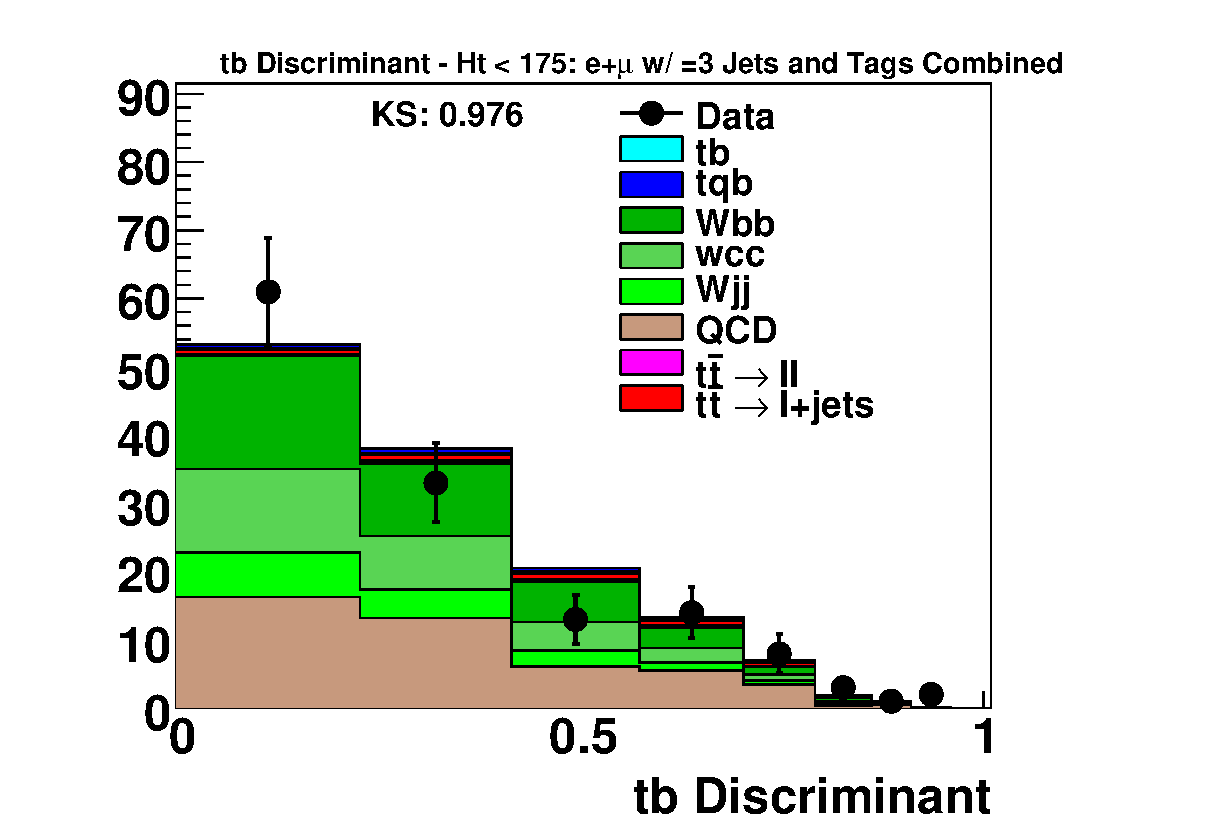
\includegraphics[width=0.49\textwidth]
{eps/MatrixElement/cross_check/combined/3jet/Wjets_tb_Discriminant}
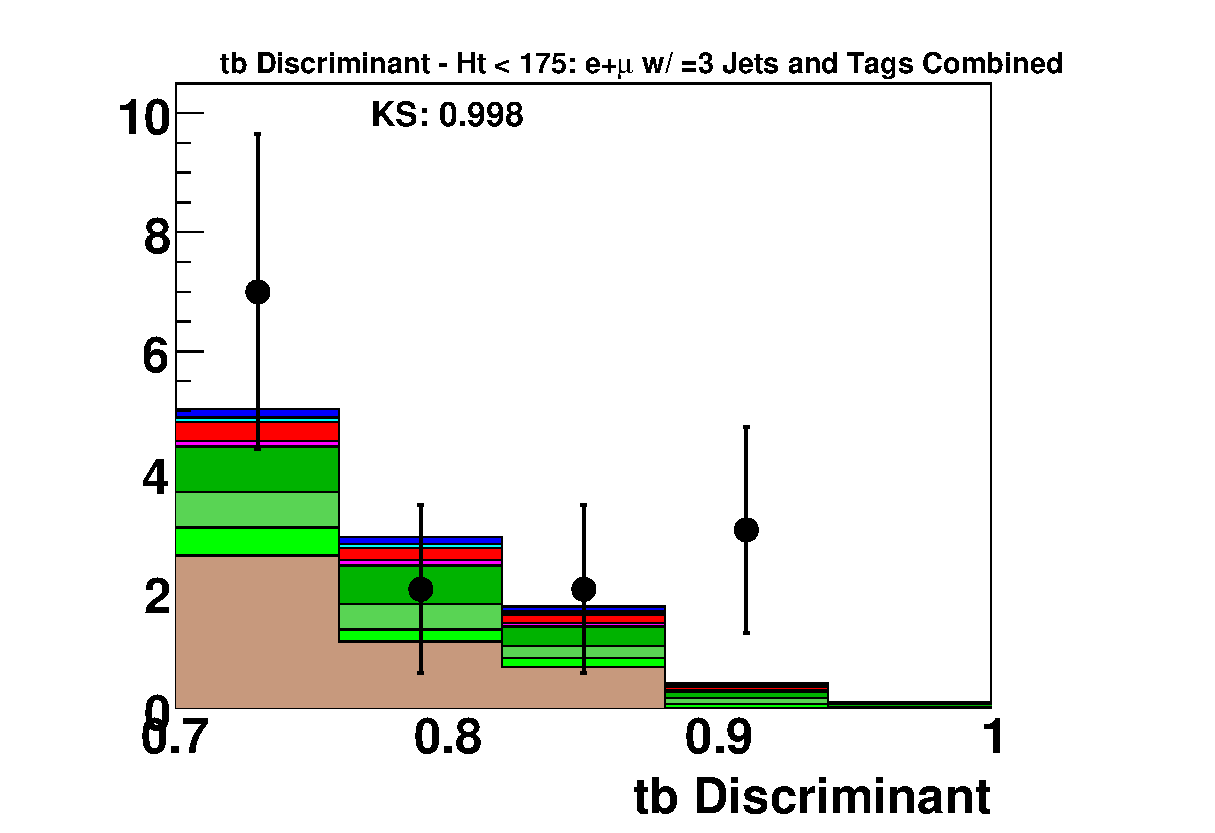
\includegraphics[width=0.49\textwidth]
{eps/MatrixElement/cross_check/combined/3jet/Wjets_tb_Discriminant_Zoom}
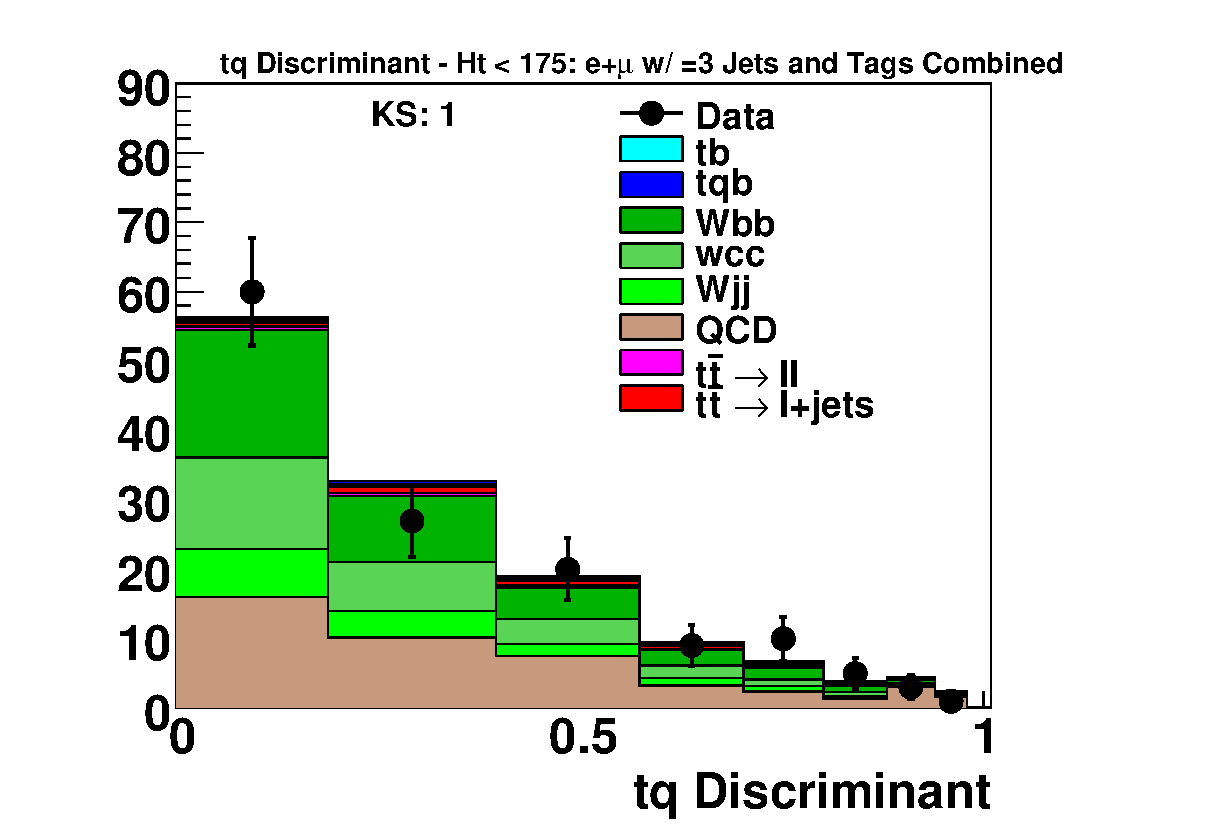
\includegraphics[width=0.49\textwidth]
{eps/MatrixElement/cross_check/combined/3jet/Wjets_tq_Discriminant}
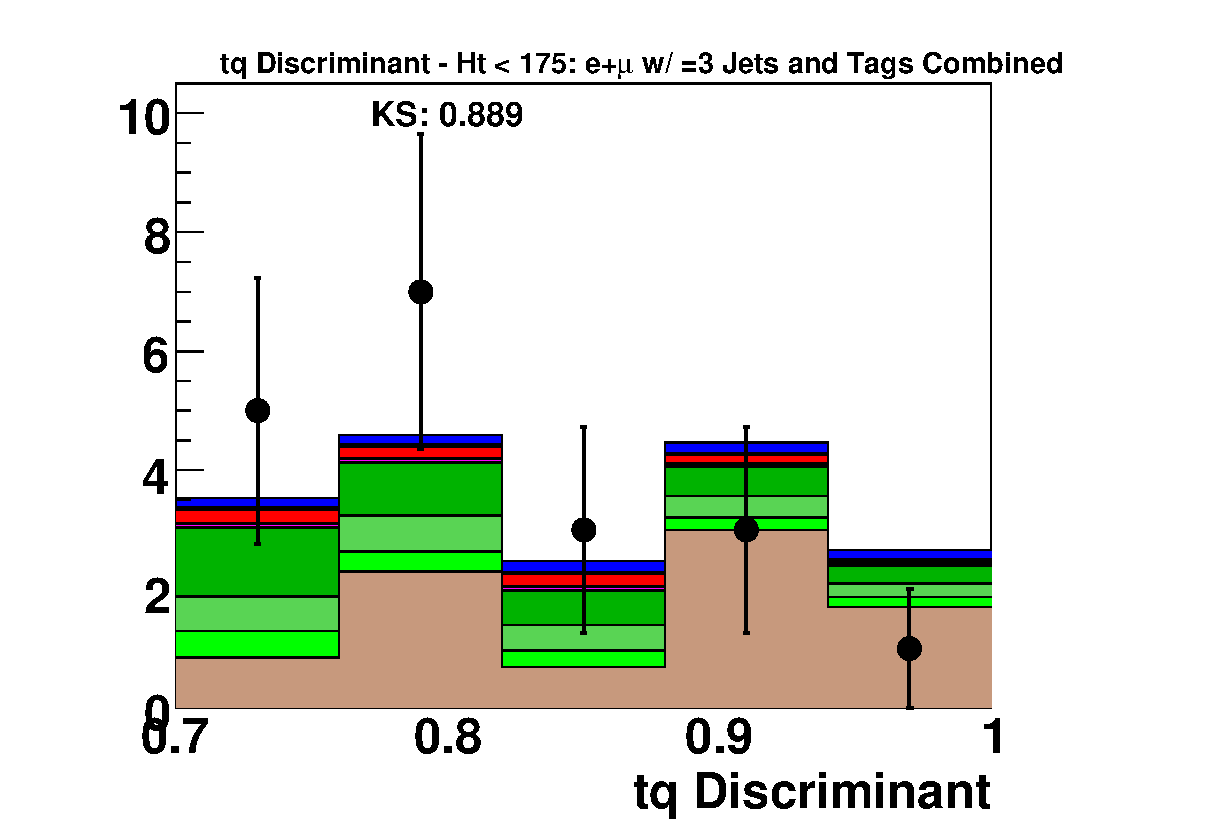
\includegraphics[width=0.49\textwidth]
{eps/MatrixElement/cross_check/combined/3jet/Wjets_tq_Discriminant_Zoom}
\vspace{-0.1in}
\caption{``Soft $W$+jets'' cross-check plots in three-jet
events for the $tb$ discriminant (upper row) and the $tq$ discriminant
(lower row). The left column shows the full discriminant region while
the right column shows the high discriminant region above 0.7.}
\label{wjets-cross-3jet}
\end{figure}

\clearpage
\begin{figure}[!h!tbp]
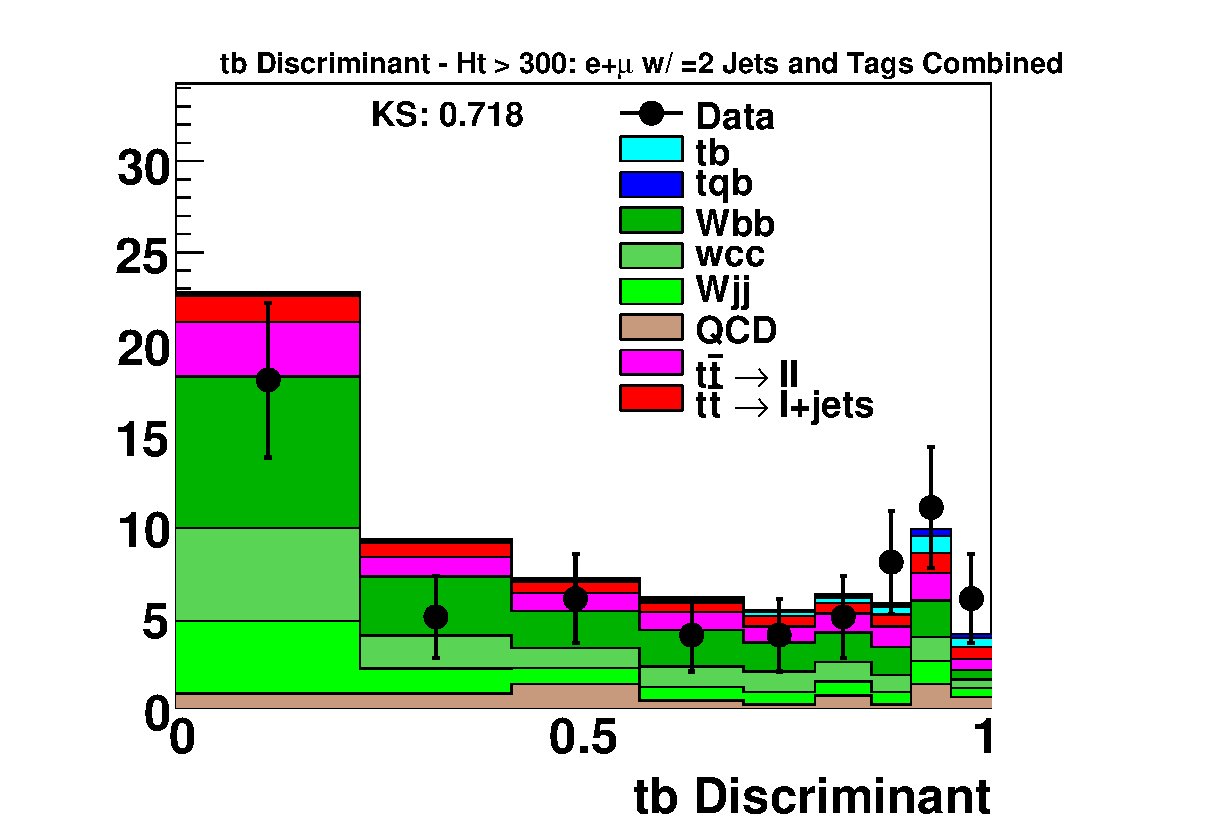
\includegraphics[width=0.49\textwidth]
{eps/MatrixElement/cross_check/combined/2jet/TTbar_tb_Discriminant}
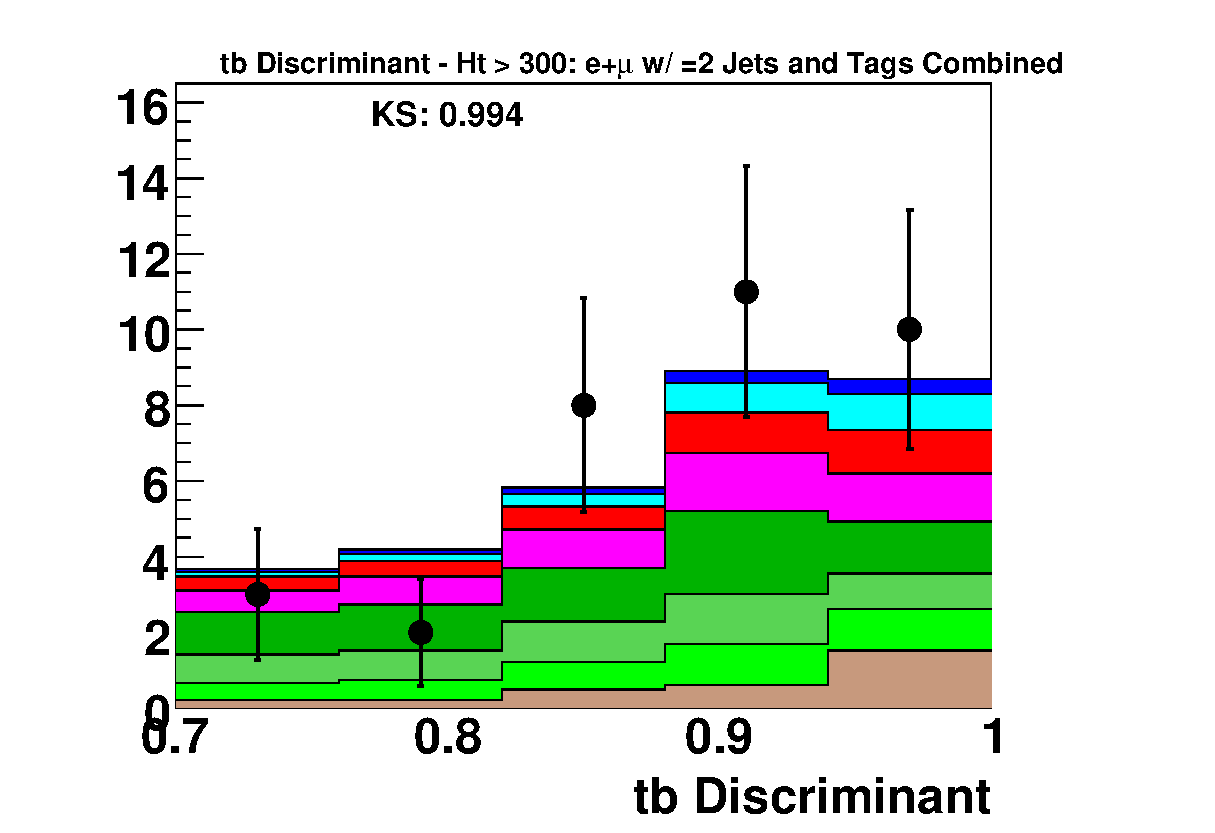
\includegraphics[width=0.49\textwidth]
{eps/MatrixElement/cross_check/combined/2jet/TTbar_tb_Discriminant_Zoom}
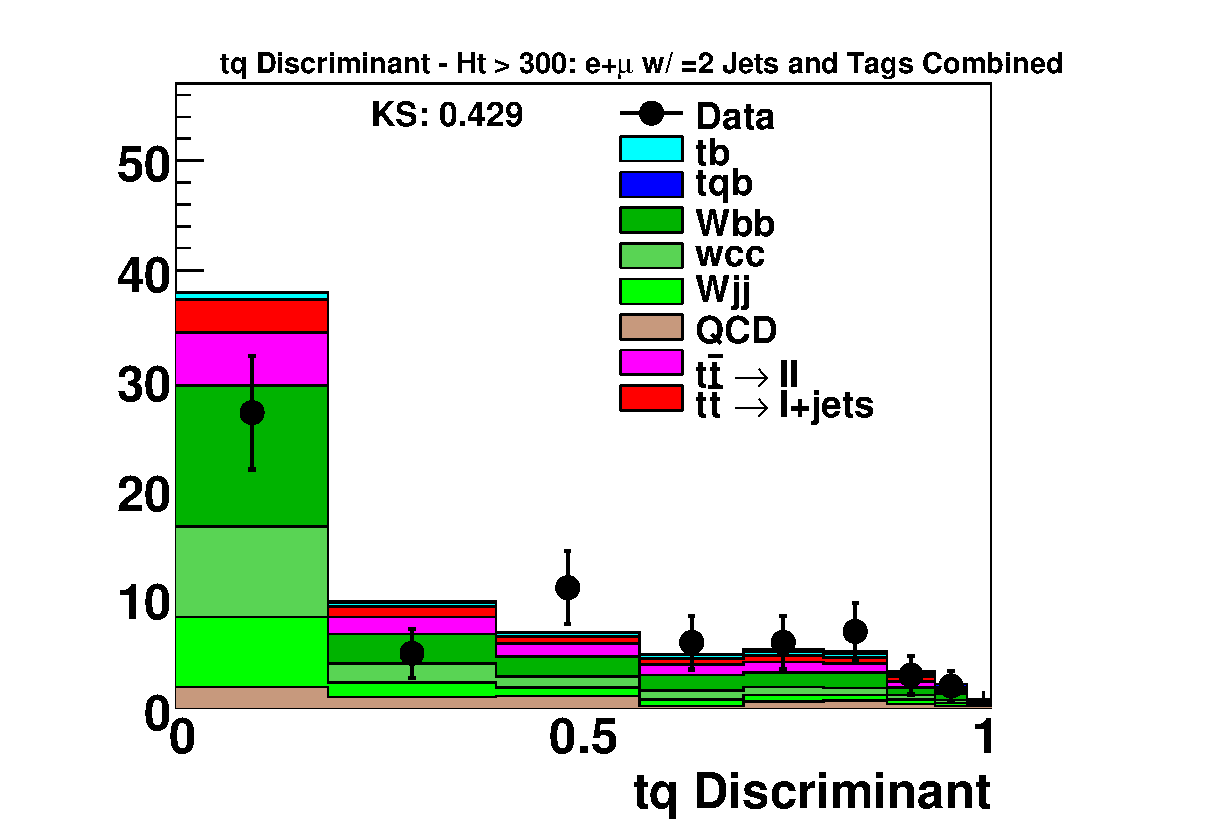
\includegraphics[width=0.49\textwidth]
{eps/MatrixElement/cross_check/combined/2jet/TTbar_tq_Discriminant}
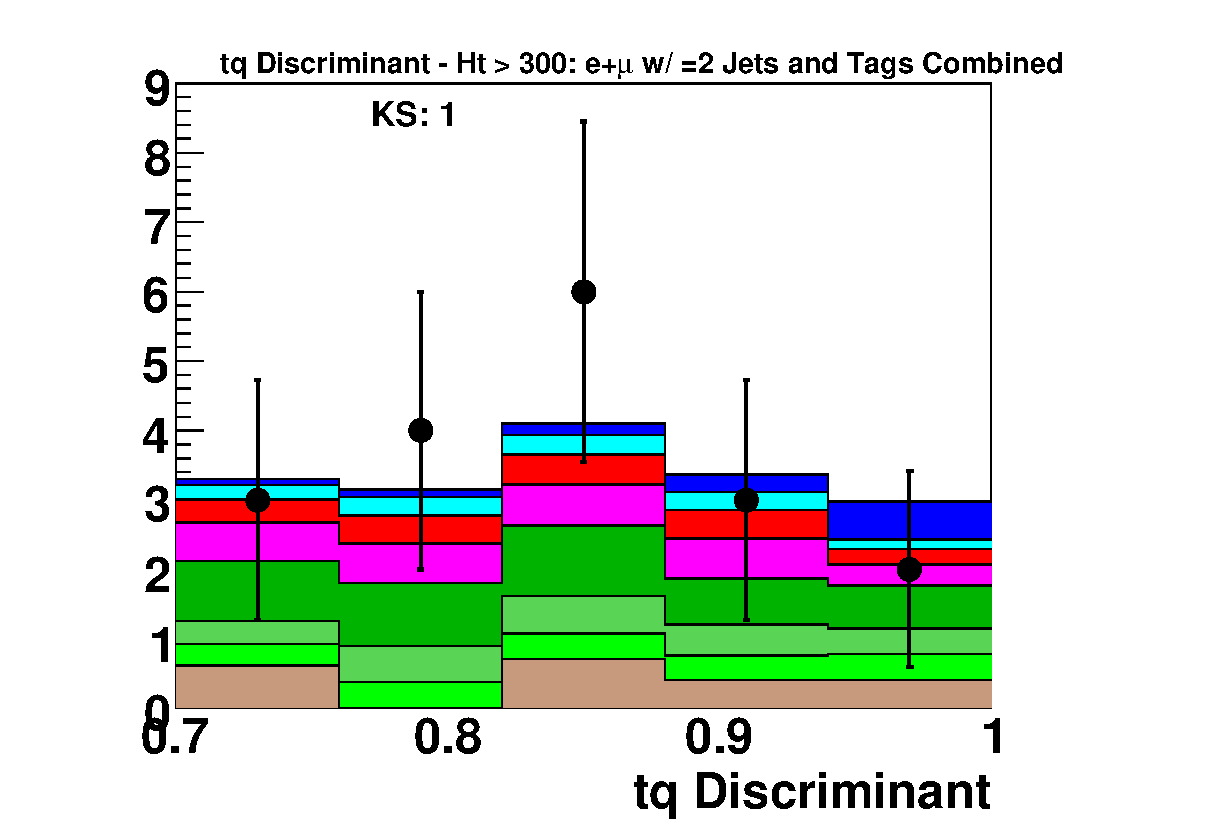
\includegraphics[width=0.49\textwidth]
{eps/MatrixElement/cross_check/combined/2jet/TTbar_tq_Discriminant_Zoom}
\vspace{-0.1in}
\caption{``Hard $W$+jets'' cross-check plots in two-jet
events for the $tb$ discriminant (upper row) and the $tq$ discriminant
(lower row). The left column shows the full discriminant region while
the right column shows the high discriminant region above 0.7.}
\label{ttbar-cross-2jet}
\end{figure}

\clearpage
\begin{figure}[!h!tbp]
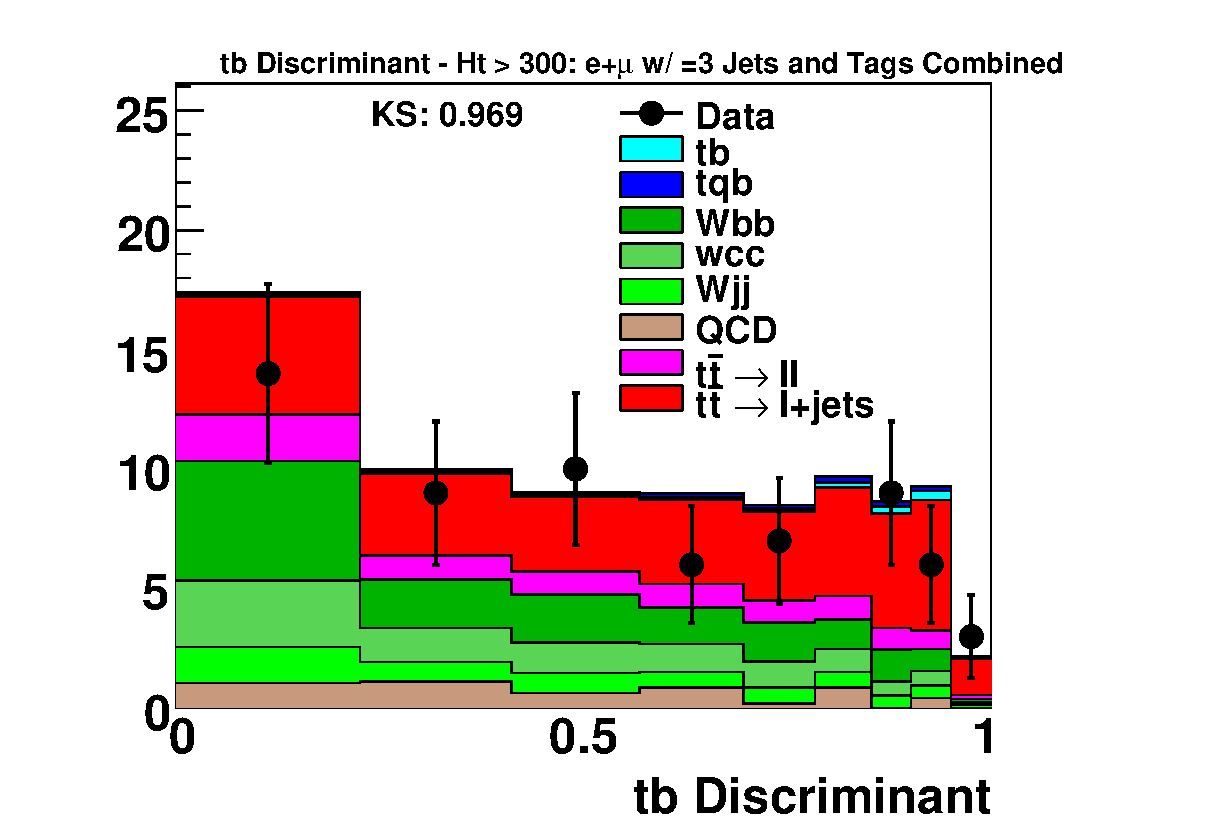
\includegraphics[width=0.49\textwidth]
{eps/MatrixElement/cross_check/combined/3jet/TTbar_tb_Discriminant}
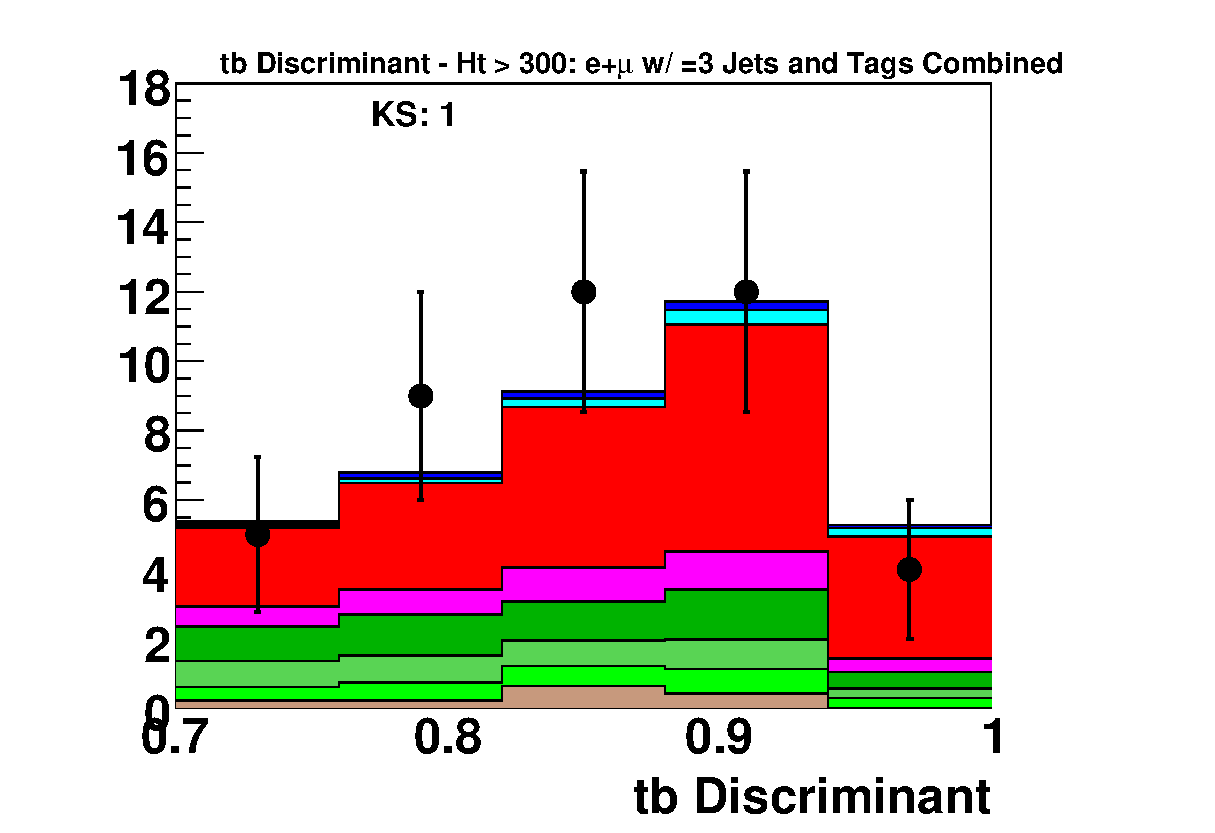
\includegraphics[width=0.49\textwidth]
{eps/MatrixElement/cross_check/combined/3jet/TTbar_tb_Discriminant_Zoom}
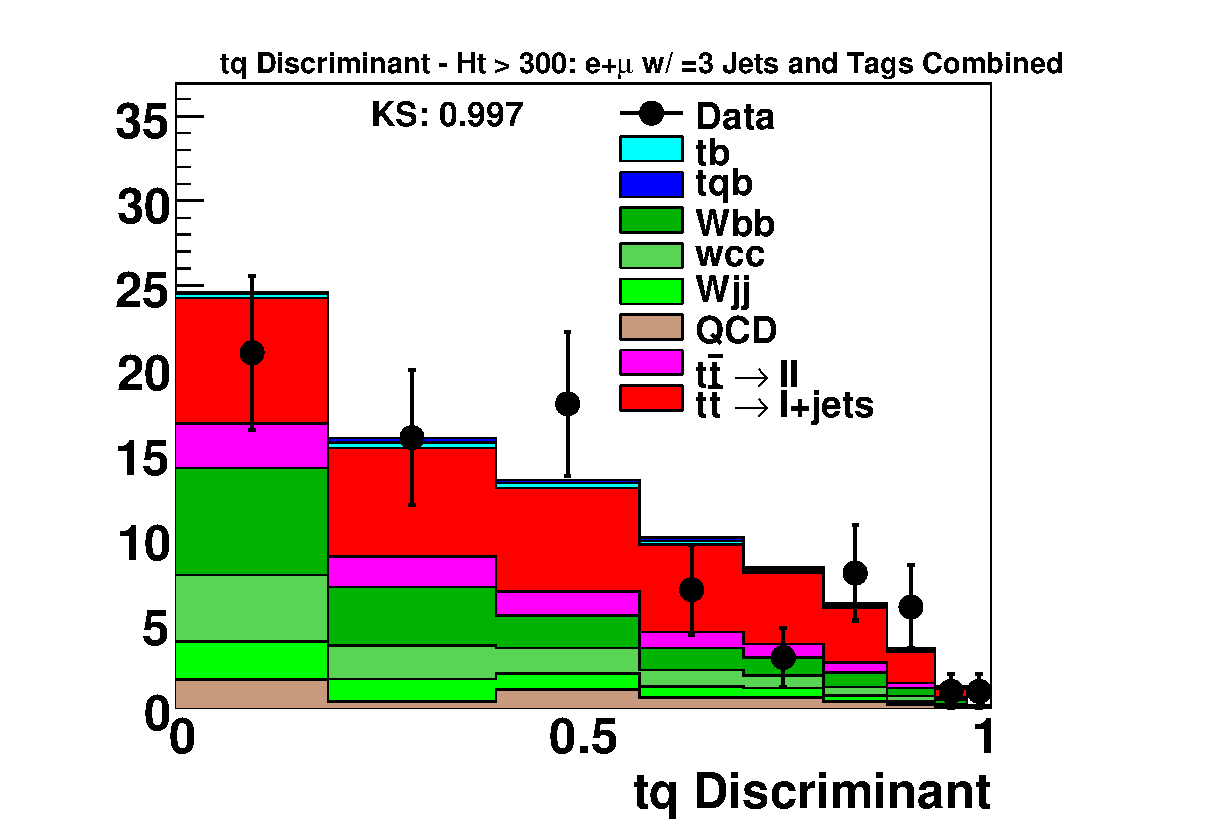
\includegraphics[width=0.49\textwidth]
{eps/MatrixElement/cross_check/combined/3jet/TTbar_tq_Discriminant}
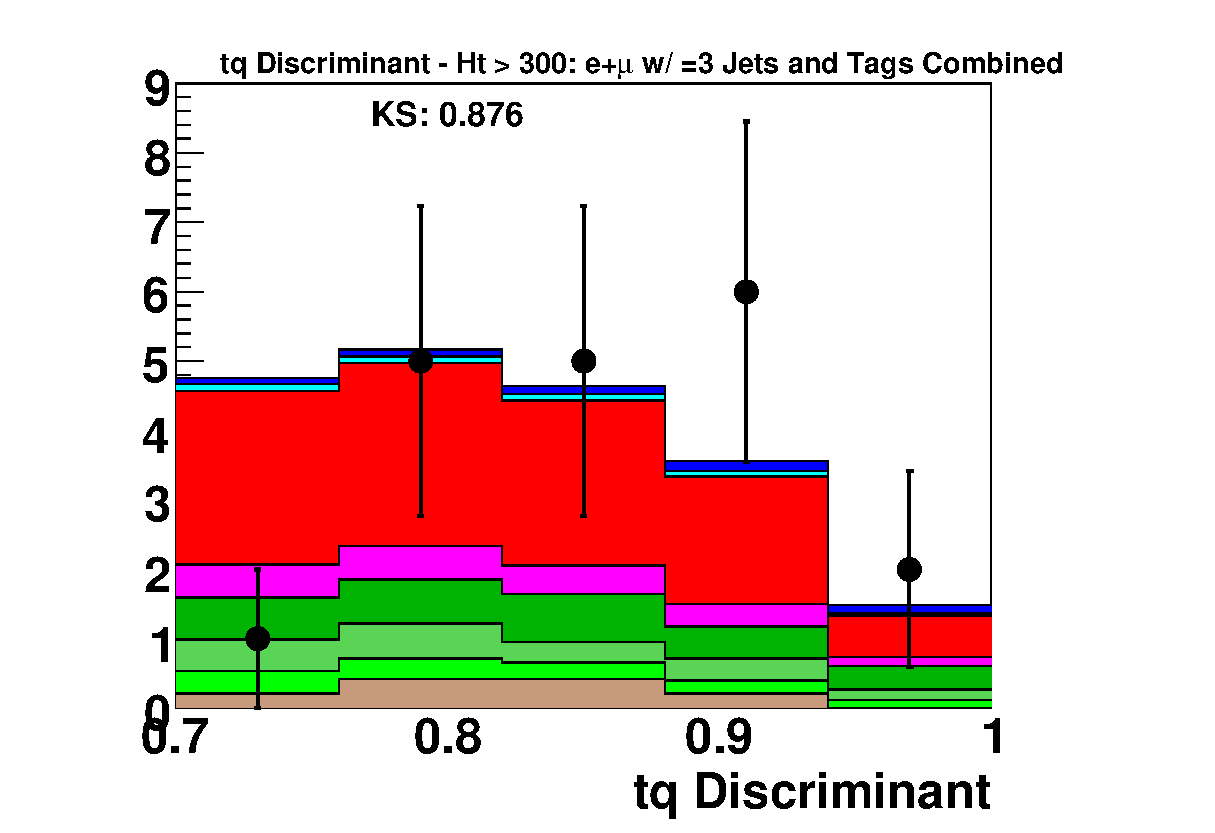
\includegraphics[width=0.49\textwidth]
{eps/MatrixElement/cross_check/combined/3jet/TTbar_tq_Discriminant_Zoom}
\vspace{-0.1in}
\caption{``Hard $W$+jets'' cross-check plots in three-jet
events for the $tb$ discriminant (upper row) and the $tq$ discriminant
(lower row). The left column shows the full discriminant region while
the right column shows the high discriminant region above 0.7.}
\label{ttbar-cross-3jet}
\end{figure}

\clearpage
\section{Matrix Element Discriminants}
\label{matrixelementresults}

This section presents the matrix element discriminants for all events in each analysis channel. Figures~\ref{e21_2j} and~\ref{e21_3j} show the $tb$ and $tqb$
discriminants for the combined $e$,$\mu$ w/ $\geq1$ $B$-tag events for two-jet
and three-jet events where the data distributions may be compared to
the background model.  The SM prediction for single top quark
production has been added to the background sum in the plots. The
individual channel plots for the 1D discriminants are shown in
Appendix~\ref{Channel}.

\vspace{-0.05in}
\begin{figure}[!h!tbp]
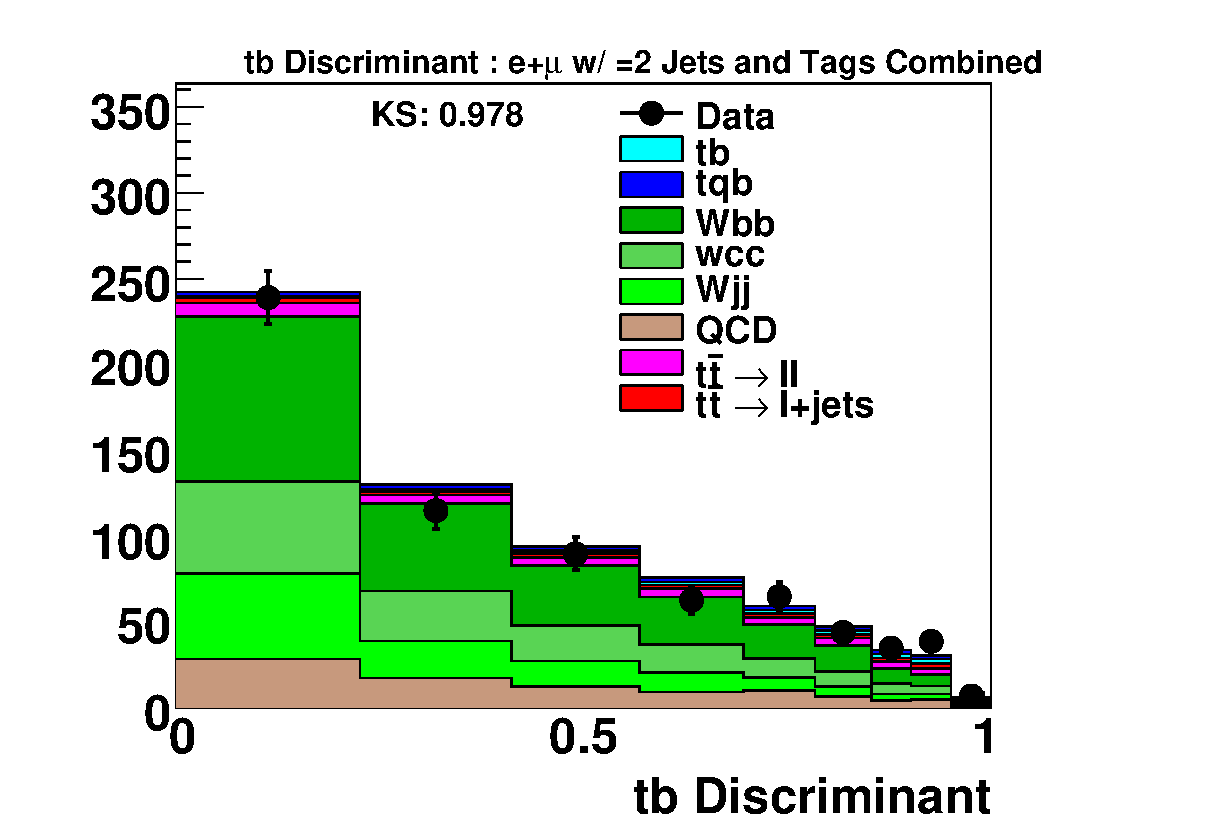
\includegraphics[width=0.49\textwidth]
{eps/MatrixElement/output/2jet/All_tb_Discriminant.eps}
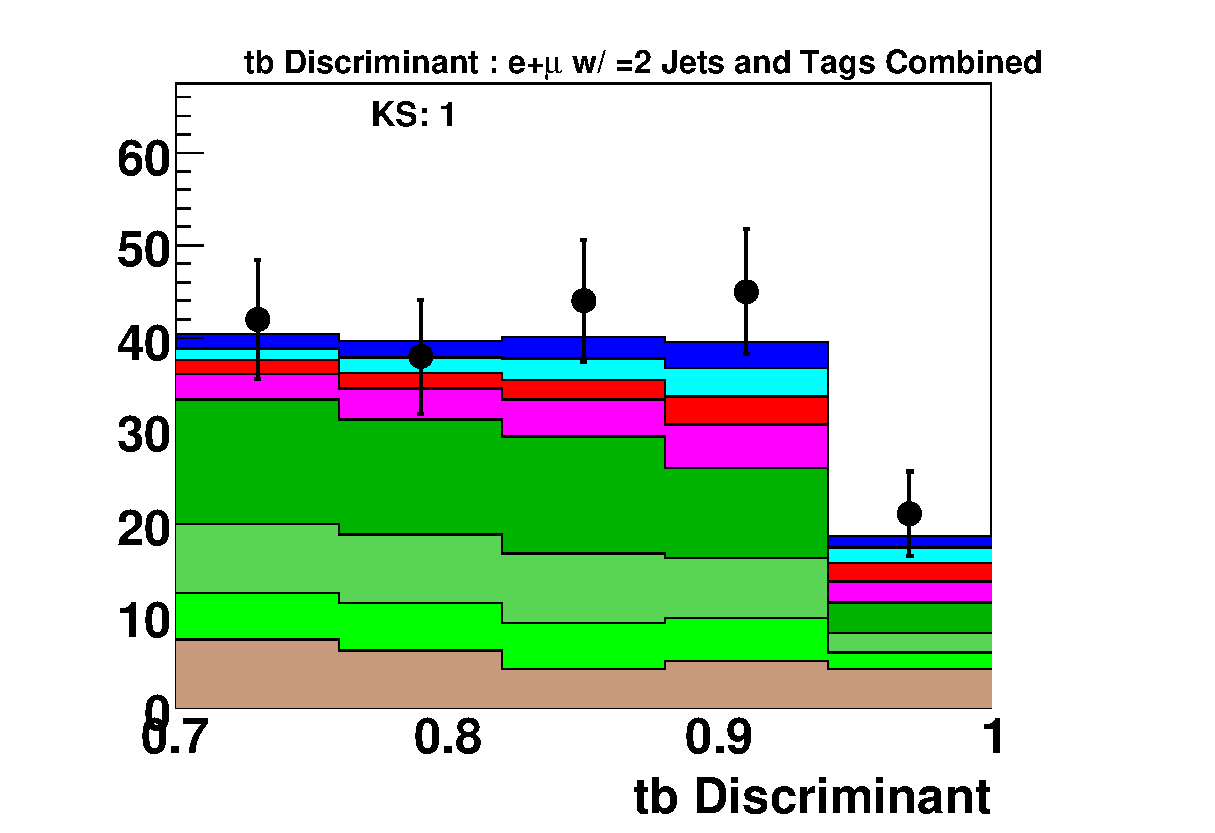
\includegraphics[width=0.49\textwidth]
{eps/MatrixElement/output/2jet/All_tb_Discriminant_Zoom.eps}
\includegraphics[width=0.49\textwidth]
{eps/MatrixElement/output/2jet/All_tq_Discriminant.eps}
\includegraphics[width=0.49\textwidth]
{eps/MatrixElement/output/2jet/All_tq_Discriminant_Zoom.eps}
\vspace{-0.1in}
\caption{Discriminant plots for the e+$\mu$ channel with two jets and
$\geq$~1 $B$~tag. Upper row: $tb$ discriminant; lower row: $tq$
discriminant. Left column: full output range; right column: close-up
of the high end of the distributions.}
\label{e21_2j}
\end{figure}

\vspace{-0.05in}
\begin{figure}[!h!tbp]
\includegraphics[width=0.49\textwidth]
{eps/MatrixElement/output/3jet/All_tb_Discriminant.eps}
\includegraphics[width=0.49\textwidth]
{eps/MatrixElement/output/3jet/All_tb_Discriminant_Zoom.eps}
\includegraphics[width=0.49\textwidth]
{eps/MatrixElement/output/3jet/All_tq_Discriminant.eps}
\includegraphics[width=0.49\textwidth]
{eps/MatrixElement/output/3jet/All_tq_Discriminant_Zoom.eps}
\vspace{-0.1in}
\caption{Discriminant plots for the e+$\mu$ channel with three jets
and $\geq$~1 $b$~tag. Upper row: $tb$ discriminant; lower row: $tq$
discriminant. Left column: full output range; right column: close-up
of the high end of the distributions.}
\label{e21_3j}
\end{figure}

After the matrix element discriminant has been calculated, it is
possible to place a cut on this value to select events in data and
Monte Carlo to see if they are consistent with single top quark
production. For this section, an event is considered very single top
quark like if both the $s$-channel and $t$-channel discriminants are
greater than 0.7. Similarly, an event is considered background like if
both discriminants are less than 0.4. Figure~\ref{top-mass} shows the
invariant mass of the lepton, neutrino, and tagged jet before and
after the discriminant cut, and Fig.~\ref{q-eta} shows the
lepton-charge times pseudorapidity of the untagged jet.

\begin{figure}[!h!tbp]
\includegraphics[width=0.49\textwidth]
{eps/MatrixElement/topovars/BTaggedTopMass_0.eps}
\includegraphics[width=0.49\textwidth]
{eps/MatrixElement/topovars/BTaggedTopMass_-0.4.eps}
\includegraphics[width=0.49\textwidth]
{eps/MatrixElement/topovars/BTaggedTopMass_0.7.eps}
\vspace{-0.1in}
\caption{Invariant mass of the lepton, neutrino, and tagged
jet for all events (upper left plot), for events with $D < 0.4$ (upper right plot), and events with $D > 0.7$ (bottom left plot).}
\label{top-mass}
\end{figure}

%\vspace{0.1in}
\begin{figure}[!h!tbp]
\includegraphics[width=0.49\textwidth]
{eps/MatrixElement/topovars/QTimesEta_0.eps}
\includegraphics[width=0.49\textwidth]
{eps/MatrixElement/topovars/QTimesEta_-0.4.eps}
\includegraphics[width=0.49\textwidth]
{eps/MatrixElement/topovars/QTimesEta_0.7.eps}
\vspace{-0.1in}
\caption{Lepton charge times the pseudorapidity of the untagged
jet for all events (upper left plot), for events with $D < 0.4$ (upper right
plot), and events with $D > 0.7$ (bottom left plot). The number of observed
events is different from the $b$-tagged top mass plot because this
variable is only defined for events with at least one untagged jet.}
\label{q-eta}
\end{figure}
